\documentclass[]{elsarticle} %review=doublespace preprint=single 5p=2 column
%%% Begin My package additions %%%%%%%%%%%%%%%%%%%
\usepackage[hyphens]{url}



\usepackage{lineno} % add
\providecommand{\tightlist}{%
  \setlength{\itemsep}{0pt}\setlength{\parskip}{0pt}}

\usepackage{graphicx}
\usepackage{booktabs} % book-quality tables
%%%%%%%%%%%%%%%% end my additions to header

\usepackage[T1]{fontenc}
\usepackage{lmodern}
\usepackage{amssymb,amsmath}
\usepackage{ifxetex,ifluatex}
\usepackage{fixltx2e} % provides \textsubscript
% use upquote if available, for straight quotes in verbatim environments
\IfFileExists{upquote.sty}{\usepackage{upquote}}{}
\ifnum 0\ifxetex 1\fi\ifluatex 1\fi=0 % if pdftex
  \usepackage[utf8]{inputenc}
\else % if luatex or xelatex
  \usepackage{fontspec}
  \ifxetex
    \usepackage{xltxtra,xunicode}
  \fi
  \defaultfontfeatures{Mapping=tex-text,Scale=MatchLowercase}
  \newcommand{\euro}{€}
\fi
% use microtype if available
\IfFileExists{microtype.sty}{\usepackage{microtype}}{}
\usepackage[left=3cm,right=3cm,top=3cm,bottom=3cm]{geometry}
\bibliographystyle{elsarticle-harv}
\usepackage{longtable}
\ifxetex
  \usepackage[setpagesize=false, % page size defined by xetex
              unicode=false, % unicode breaks when used with xetex
              xetex]{hyperref}
\else
  \usepackage[unicode=true]{hyperref}
\fi
\hypersetup{breaklinks=true,
            bookmarks=true,
            pdfauthor={},
            pdftitle={Living on the edge: crop boundary effects on canola and wheat yields in Alberta},
            colorlinks=false,
            urlcolor=blue,
            linkcolor=magenta,
            pdfborder={0 0 0}}
\urlstyle{same}  % don't use monospace font for urls

\setcounter{secnumdepth}{5}
% Pandoc toggle for numbering sections (defaults to be off)

% Pandoc citation processing
\newlength{\csllabelwidth}
\setlength{\csllabelwidth}{3em}
\newlength{\cslhangindent}
\setlength{\cslhangindent}{1.5em}
% for Pandoc 2.8 to 2.10.1
\newenvironment{cslreferences}%
  {}%
  {\par}
% For Pandoc 2.11+
\newenvironment{CSLReferences}[3] % #1 hanging-ident, #2 entry spacing
 {% don't indent paragraphs
  \setlength{\parindent}{0pt}
  % turn on hanging indent if param 1 is 1
  \ifodd #1 \everypar{\setlength{\hangindent}{\cslhangindent}}\ignorespaces\fi
  % set entry spacing
  \ifnum #2 > 0
  \setlength{\parskip}{#2\baselineskip}
  \fi
 }%
 {}
\usepackage{calc} % for calculating minipage widths
\newcommand{\CSLBlock}[1]{#1\hfill\break}
\newcommand{\CSLLeftMargin}[1]{\parbox[t]{\csllabelwidth}{#1}}
\newcommand{\CSLRightInline}[1]{\parbox[t]{\linewidth - \csllabelwidth}{#1}}
\newcommand{\CSLIndent}[1]{\hspace{\cslhangindent}#1}

% Pandoc header
\makeatletter \def\ps@pprintTitle{  \let\@oddhead\@empty  \let\@evenhead\@empty  \def\@oddfoot{\centerline{\thepage}} \let\@evenfoot\@oddfoot} \makeatother \usepackage{float} \floatplacement{figure}{H} \newcommand{\beginsupplement}{\setcounter{table}{0} \renewcommand{\thetable}{S\arabic{table}} \setcounter{figure}{0} \renewcommand{\thefigure}{S\arabic{figure}}} \usepackage{setspace} \linenumbers
\usepackage{booktabs}
\usepackage{longtable}
\usepackage{array}
\usepackage{multirow}
\usepackage{wrapfig}
\usepackage{float}
\usepackage{colortbl}
\usepackage{pdflscape}
\usepackage{tabu}
\usepackage{threeparttable}
\usepackage{threeparttablex}
\usepackage[normalem]{ulem}
\usepackage{makecell}
\usepackage{xcolor}



\begin{document}
\begin{frontmatter}

  \title{Living on the edge: crop boundary effects on canola and wheat yields in Alberta}
    \author[University of Calgary]{Samuel V. J. Robinson\corref{1}}
   \ead{samuel.robinson@ucalgary.ca} 
    \author[University of Calgary]{Lan H. Nguyen}
   \ead{hoanglan.nguyen@ucalgary.ca} 
    \author[University of Calgary]{Paul Galpern}
   \ead{paul.galpern@ucalgary.ca} 
      \address[University of Calgary]{2500 University Drive NW, Calgary, AB}
      \cortext[1]{Corresponding Author}
  
  \begin{abstract}
  Field boundaries can improve crop yields by creating better abiotic conditions for crop growth (e.g.~mosture, temperature), and can act as refuges for beneficial arthropods. This suggests that beneficial crop boundaries may create an intermediate hump-shaped increase in crop yield, where negative edge effects are cancelled out by increased ecosystem services (e.g.~pollination or pest suppression) from the field boundary. However, there is little large-scale evidence showing this, largely because yield is costly and time-consuming to measure. Precision yield data from combine yield monitors has huge potential in this respect, as the equipment is relatively cheap and commonly measured by growers. Average crop yield tended to increase with distance from crop boundaries before plateauing at about 50 m, and yield variation (SD) tended to decrease concurrently with distance. Differences between boundary types tended to be weak and variable, especially for wheat; there was some evidence of certain field boundaries causing a greater decrease in yield at the edge, but these differences tended to be small in magnitude (\textless5\% of yield). Furthermore, there was little evidence of an intermediate increase in yield, suggesting that a) ecosystem services do not strongly depend on distance or b) their effect is relatively small. This study represents one of the first uses of precision yield data to measure ecosystem service provision at large spatial scales.
  \end{abstract}
   \begin{keyword} precision yield; spillover; landscape;\end{keyword}
 \end{frontmatter}

Potential journals: Agriculture Ecosystems and Environment, Basic and Applied Ecology, Ecological Economics, Journal of Applied Ecology (probably won't like it)

Potential reviewers: Teja Tscharntke, Ignasi Bartomeus, Ben Woodcock, John Redhead, some Canadian/Albertan reviewers who know the crop systems?

\newpage
\doublespacing

\hypertarget{introduction}{%
\section{Introduction}\label{introduction}}

Intensive agricultural production has increased over the last 100 years, and agricultural land now makes up over a third of ice-free land on Earth.
This has allowed increases in human population and increased global stability in production.
However, this is not without cost, as higher-diversity non-crops are converted to lower-diversity crops, resulting in loss of habitat and overall biodiversity of non-target organisms.
Maintaining both biodiversity and production in agroecosystems represents a seldom-considered goal of conservationists and agronomists, and hold the potential for win-win scenarios.
Key to this is the preservation of semi-natural land (SNL), which represents the interface between crops and non-crops within agroecosystems.

SNL in and around crops is important for both agricultural production and conservation (Prieto-Benítez \& Méndez 2011), as it has the potential to create better biotic and abiotic conditions for crop growth (Case \emph{et al.} 2019; Weninger \emph{et al.} 2021; but see Lowe \emph{et al.} 2021).
They are habitat for mobile organisms, and can act as sources of ecosystem services such as pollination or pest control (Albrecht \emph{et al.} 2020; Gardner \emph{et al.} 2021), but this can vary depending on the system (Gray \& Lewis 2014; Quinn \emph{et al.} 2017)
They also can create microclimate effects that reduce extreme temperature, trap moisture, and reduce wind speed (Kort 1988; Brandle \emph{et al.} 2004).
North American agroecosystems have larger fields, different crop varieties, and agronomic practices, all of which could negate or confound potential effects of SNL

SNL may affect yields at intermediate distances, depending on the spatial scale at which ecosystem services operate.
Edge effects cause low yields at the edge of crops because of sparse or late seedling emergence, poor microclimate, and competition with weeds.
At the same time, the centre of large fields will not receive ecosystem services if they decay with distance from edges (Kowalchuk \& Jong 1995).
For example, pollination services from central place foragers (bees) that nest in SNL but forage in crops drops rapidly with distance (Garibaldi \emph{et al.} 2011).
Therefore, yield may be maximized at intermediate distances, where the ecosystem services cancel out negative edge effects (Van Vooren \emph{et al.} 2017).
This suggests a ``goldilocks'' field size, where negative edge effects are canceled out by ecosystem services.

\begin{figure}
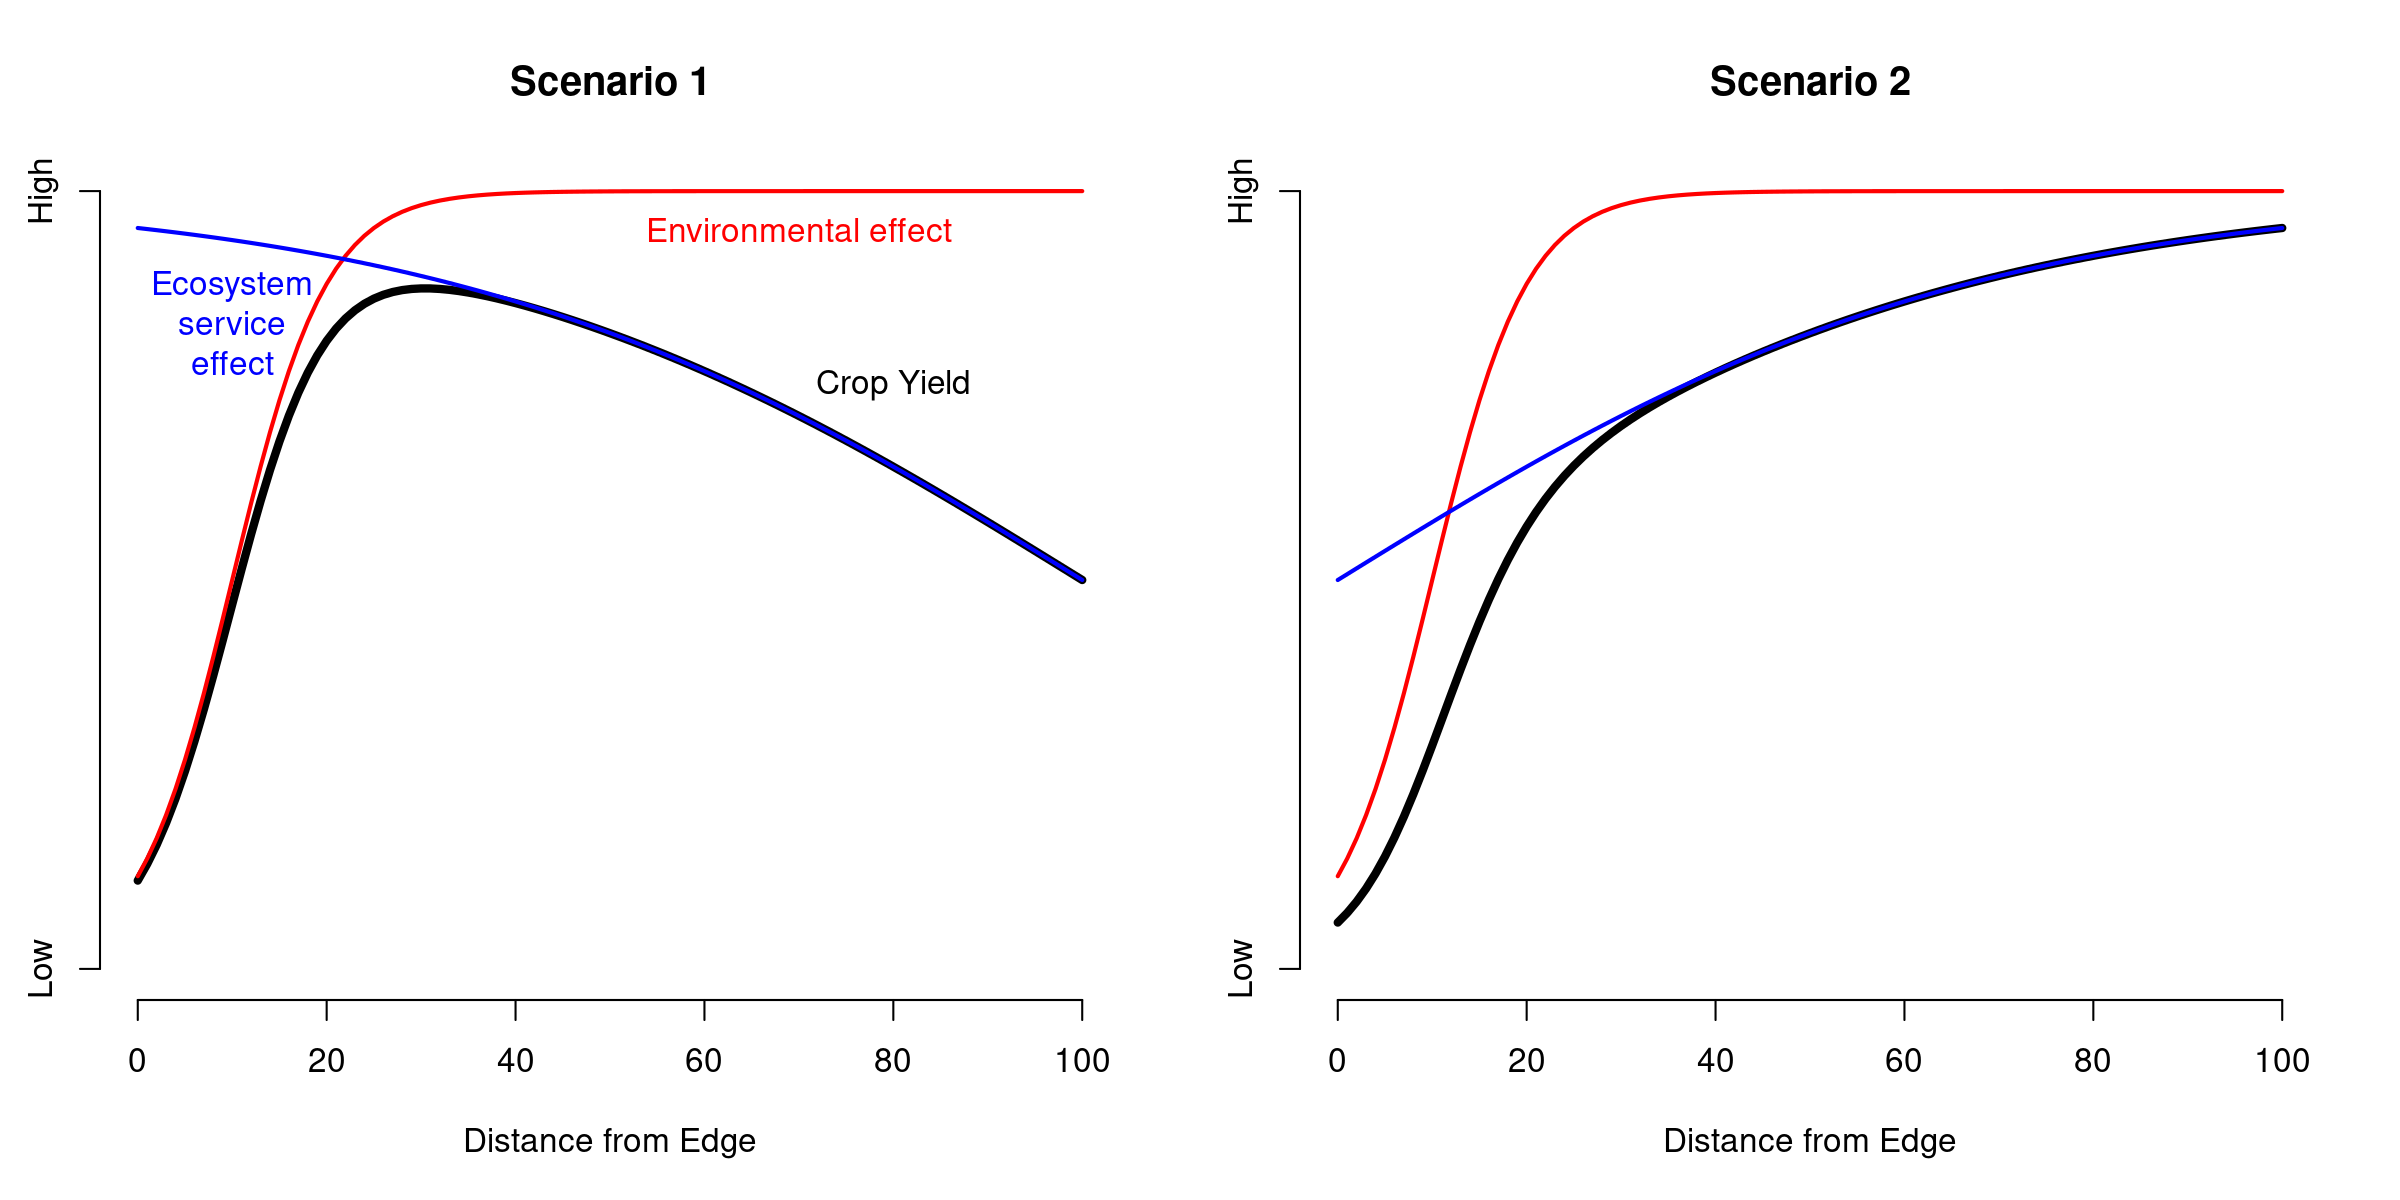
\includegraphics[width=1\linewidth]{../Figures/ExamplePlots/hypotheses} \caption{Potential yield patterns, depending on ecosystem service effects with distance. In both figures, negative environmental effects (edge effects) are shown in red, and decrease with distance from the edge of the crop, creating an increase in yield with distance. The left figure shows a decline in ecosystem services with distance, leading to an intermediate peak in yield, while the right figure shows an increase in services with distance, leading to a peak at the centre of the field (note: Scenario 2 also occurs if ecosystem services do not change with distance).}\label{fig:hypotheses}
\end{figure}

Studies of SNL effects on crop yield also suffer from limited scope (e.g.~few crop types) and small sample sizes, limiting inference and reducing generality (Baker \emph{et al.} 2018; but see also Redhead \emph{et al.} 2020).
Meta-analyses have been the standard solution to this problem (e.g. Albrecht \emph{et al.} 2020; Lowe \emph{et al.} 2021), but precision yield data holds enormous promise.
However, its use is limited for several reasons, namely: 1) Lack of standardized formats between equipment types, 2) Sensor calibration required for field-level accuracy, and 3) low familiarity with spatial statistics.
Ecosystem services can influence both the mean and variability of yield in agroecosystems (Redhead \emph{et al.} 2020); typically only averages (means) are considered, but higher stability (lower variance) in yield can also be valuable from a grower's perspective.
There are few studies of yield variability (only those with large datasets), but precision yield data opens up the possibility of modeling within-field variability, as well as average yield.

In this paper we ask:
1. How does crop yield change with distance from the edge of field?
2. Does this depend on type of field edge?
3. Is there an intermediate distance where yield is maximized or variance is minimized?
To our knowledge, no other study has addressed the effect of field boundaries on productivity using precision yield, making this study highly novel.

\hypertarget{methods}{%
\section{Methods}\label{methods}}

\hypertarget{data-collection}{%
\subsection{Data collection}\label{data-collection}}

Precision yield data were collected directly from farmers across Alberta.
Farmers were solicited for yield data through local agronomists, and we received 298 field-years of data from 5 growers across a total of 7 years (2014-2020).
We converted raw data to a standard csv format using Ag Leader SMS.
85\% of the crop types where either wheat (\emph{Triticum aestivum}), canola (\emph{Brassica napus}), or peas (\emph{Pisum sativum}), three of the most common crops in rotation in Alberta.
The remaining crop types had low replication, so we constrained our analysis to only field-years containing wheat (94), canola (119), or peas (39), for a total of 252 field-years of data.
Individual fields contained between 1 and 6 years of data (mean: 3.1), containing a total of 14.4 million data points.

Yield data was collected in rectangles of the same length as the data interval (distance = combine ground speed \(\times\) interval, typically 1 second) and the same width as the combine header (5-7 m, adjusted to account for overlap with adjacent swaths).
We extracted the size of each polygon (m\(^2\)), dry yield (tonnes), and the spatial location, and the sequence of collection (1 - end of harvest)
Because of the large number of yield rectangles per field (30-800 thousand), we used the centroid of each polygon as its location, treating areal data as point data
Seeding and application rates were constant across fields, so we did not consider inputs in our analysis
We used dry yield (tonnes of seed/hectare minus recorded crop moisture) as our measure of crop yield
Precision yield data can be highly variable and is prone to extreme outliers (both positive and negative), especially when combine ground speeds are low and at the beginning of rows
Therefore, we filtered data that lay outside the 95th percentiles of yield within each field, values less than or equal to zero, and values outside of the 95th percentiles of ground speed.
Due to the large number of data at each field, we sub-sampled to 50,000 data points per field to reduce computation time.

Field boundaries were automatically digitized using buffers from the yield data locations, then manually checked using satellite imagery from Google Earth and classified land cover data from AAFC.
Crop boundaries are flexible, and often change yearly depending on planting and emergence conditions (e.g.~flooding during some years).
Ephemeral wetlands are flooded during some years, but consist mainly of grasses during dry years, and grass boundaries can change if fields are used for as haying or pasture during crop rotation.
This makes accurate and consistent classification of field boundaries difficult.
We defined the following general categories for field boundaries:
1. Standard: grassy field edge, staging yard, or road right-of-way (grassy strip typically 5-10m wide)
2. Wetland: permanent wetland; borders are largely unchanged from year-to-year
3. Shelterbelt: permanent windbreaks, shelterbelts, remnant forests, or shrublands
4. Other crop: annual crop or pasture with little or no visible boundary between planted areas
5. Bare: unplanted, fallow, flooded area, temporary wetland (only present for a single season), staging yard, oil and gas equipment, or road without a planted boundary
6. Grassland: permanent seminatural grassland or pasture (not in rotation)

\hypertarget{analysis}{%
\subsection{Analysis}\label{analysis}}

Yield data from each field contains both random and systematic errors that must be modeled in order to reveal underlying changes in yield.
We fit an additive model of the effect of boundary distance on crop yield while accounting for within-field spatial variation and temporal variation in the data.
Crop yield can vary within a field due to soil conditions, moisture, seeding rates, herbicide application, and previous agricultural practices.
Ground speed is extremely important to yield monitor accuracy (Arslan \& Colvin 2002), with low ground speed registering higher yields.
Sensor calibration can reduce combine-level bias (such as a combine recording consistently higher/lower yields across fields), this does not address sensor drift that occurs over time.
This may be caused by sensors accumulating debris during harvest (especially in canola, pers. comm. Trent Clark), leading to changes in accuracy and bias over time.
To model this, we fit the following model to each field-year of data:

\begin{equation}
  \begin{split}
  \sqrt{yield} \sim & Normal (\mu, \sigma)\\
  \mu = & Intercept + log(\text{Polygon Size}) + f(\text{Edge Distance}, b=12)_i + \\
   & f(\text{Easting}, \text{Northing}, b=60) + f(\text{Sequence}, b=60) \\
  log(\sigma) =  & Intercept + log(\text{Polygon Size}) + f(\text{Edge Distance}, b=12)_i + \\
   & f(\text{Easting}, \text{Northing}, b=60) + f(\text{Sequence}, b=60) \\
  \end{split}
  \end{equation}

\begin{itemize}
\tightlist
\item
  where:
\end{itemize}

\begin{enumerate}
\def\labelenumi{\arabic{enumi}.}
\tightlist
\item
  Polygon Size = distance traveled \(\times\) width of header bar (\(m^2\))
\item
  Edge Distance = distance from field edge type \emph{i} (m)
\item
  Easting, Northing = distance from centre of field (m)
\item
  Sequence = order of harvest within field (1--N points)
\item
  f(x,b) = penalized thin-plate regression spline, where \emph{x} is the predictor and \emph{b} is the number of basis dimensions
\end{enumerate}

In addition to modeling edge effects (our variable of interest), this model also accounts for a) differences in harvested area, b) within-field spatial variation not related to edges, and d) shifts in combine accuracy during harvest.
Spatial or temporal variation can be modelled using a Gaussian Process Model (e.g.~Kriging, SPDE Approximations) but this was computationally unfeasible with 50,000 data points per field.
Penalized splines offer a compromise, as they account for nonlinear ``wiggly" relationships in the same way as Gaussian processes but using a reduced number of dimensions and computation time.
The number of basis dimensions was checked with the \emph{gam.check} function from \emph{mgcv}.
The relationship between polygon size and yield was modeled with a log-linear relationship with a single slope term, as this closely matched smoothed versions.
Because polygon size is not intuitive, we converted it into ground speed by regressing speed on distance traveled per polygon, then using this to back-calculate the ground speed for a given polygon size (given a fixed width of header).
All models were fit in \emph{R} using the \emph{mgcv} library (version 1.8.36, Wood 2017), and figures were created with \emph{ggplot2} and \emph{ggpubr} (versions 3.3.3, Wickham 2016; and 0.4.0, Kassambara 2020).

Despite the use of spatial and temporal smoothers, the residuals in most of the models displayed a large amount of spatial and temporal autocorrelation.
\emph{Not really sure how we can get around this. In practice, this means that SEs for all coefficients are too small (i.e.~we gathered 1000 points, but because they're spatially related, it's only equivalent to 100 points).}

To consider results from all field-level models together, we fit models independent of each other and fit an ``overall'' smoother as averages of the field-level smoothers.
However, this does not account for uncertainty in the field-level smoothers, so we used an approach similar to bootstrapping of hierarchical mixed effects models:
1. Extract single posterior sample (\emph{rnorm} in R) of smoother parameters from each field-level model using coefficient estimates and standard error
2. Use posterior sample to create a new smoother from each field
3. Fit new model of new smoothers from all fields, and save this ``meta-smoother''
4. Repeat 1000 times, and calculate coverage intervals (5-95\% percentiles) on saved meta-smoothers
This gives coverage intervals (CIs) for the ``average'' smoother while accounting for field-level variability, and is conceptually similar to a meta-analysis.
Spatial variability was not averaged between fields because differences in field geometry make it impossible to compare fields.

\hypertarget{results}{%
\section{Results}\label{results}}

\hypertarget{field-level-example}{%
\subsection{Field-level example}\label{field-level-example}}

The filtered data from each field still contained a large amount of variation, but the non-stationary additive models were able to reveal underlying yield patterns.
To illustrate this, we show the results from a single wheat field, where we show the relative impact of ground speed, harvest sequence, boundary distance, and spatial variation on both yield mean and yield SD (``patchiness'').
Figure \ref{fig:rawData} shows the raw data collected from a single field, demonstrating a large amount of variation even among the filtered data.
Combine ground speed had a large effect on both yield mean and SD, and there was also a strong effect of harvest sequence on yield mean and SD (Figure \ref{fig:orderSmooths}.
Yield mean and SD tended to decrease with distance from field boundaries, but there were no consistent differences between boundary types (Figure \ref{fig:distSmooths}.
Finally, the random spatial smoothers in Figure \ref{fig:spatialSmooths} show that yield mean and SD systematically vary within fields, likely due to moisture, elevation, or soil conditions (Figure \ref{fig:spatialSmooths}.

\begin{figure}
\includegraphics[width=0.75\linewidth]{../Figures/ExamplePlots/rawData} \caption{Example output from a single field.}\label{fig:rawData}
\end{figure}

\begin{figure}
\includegraphics[width=1\linewidth]{../Figures/ExamplePlots/orderSmooths} \caption{Ground speed and harvest sequence (random temporal variation) smoothers from a single field.}\label{fig:orderSmooths}
\end{figure}

\begin{figure}
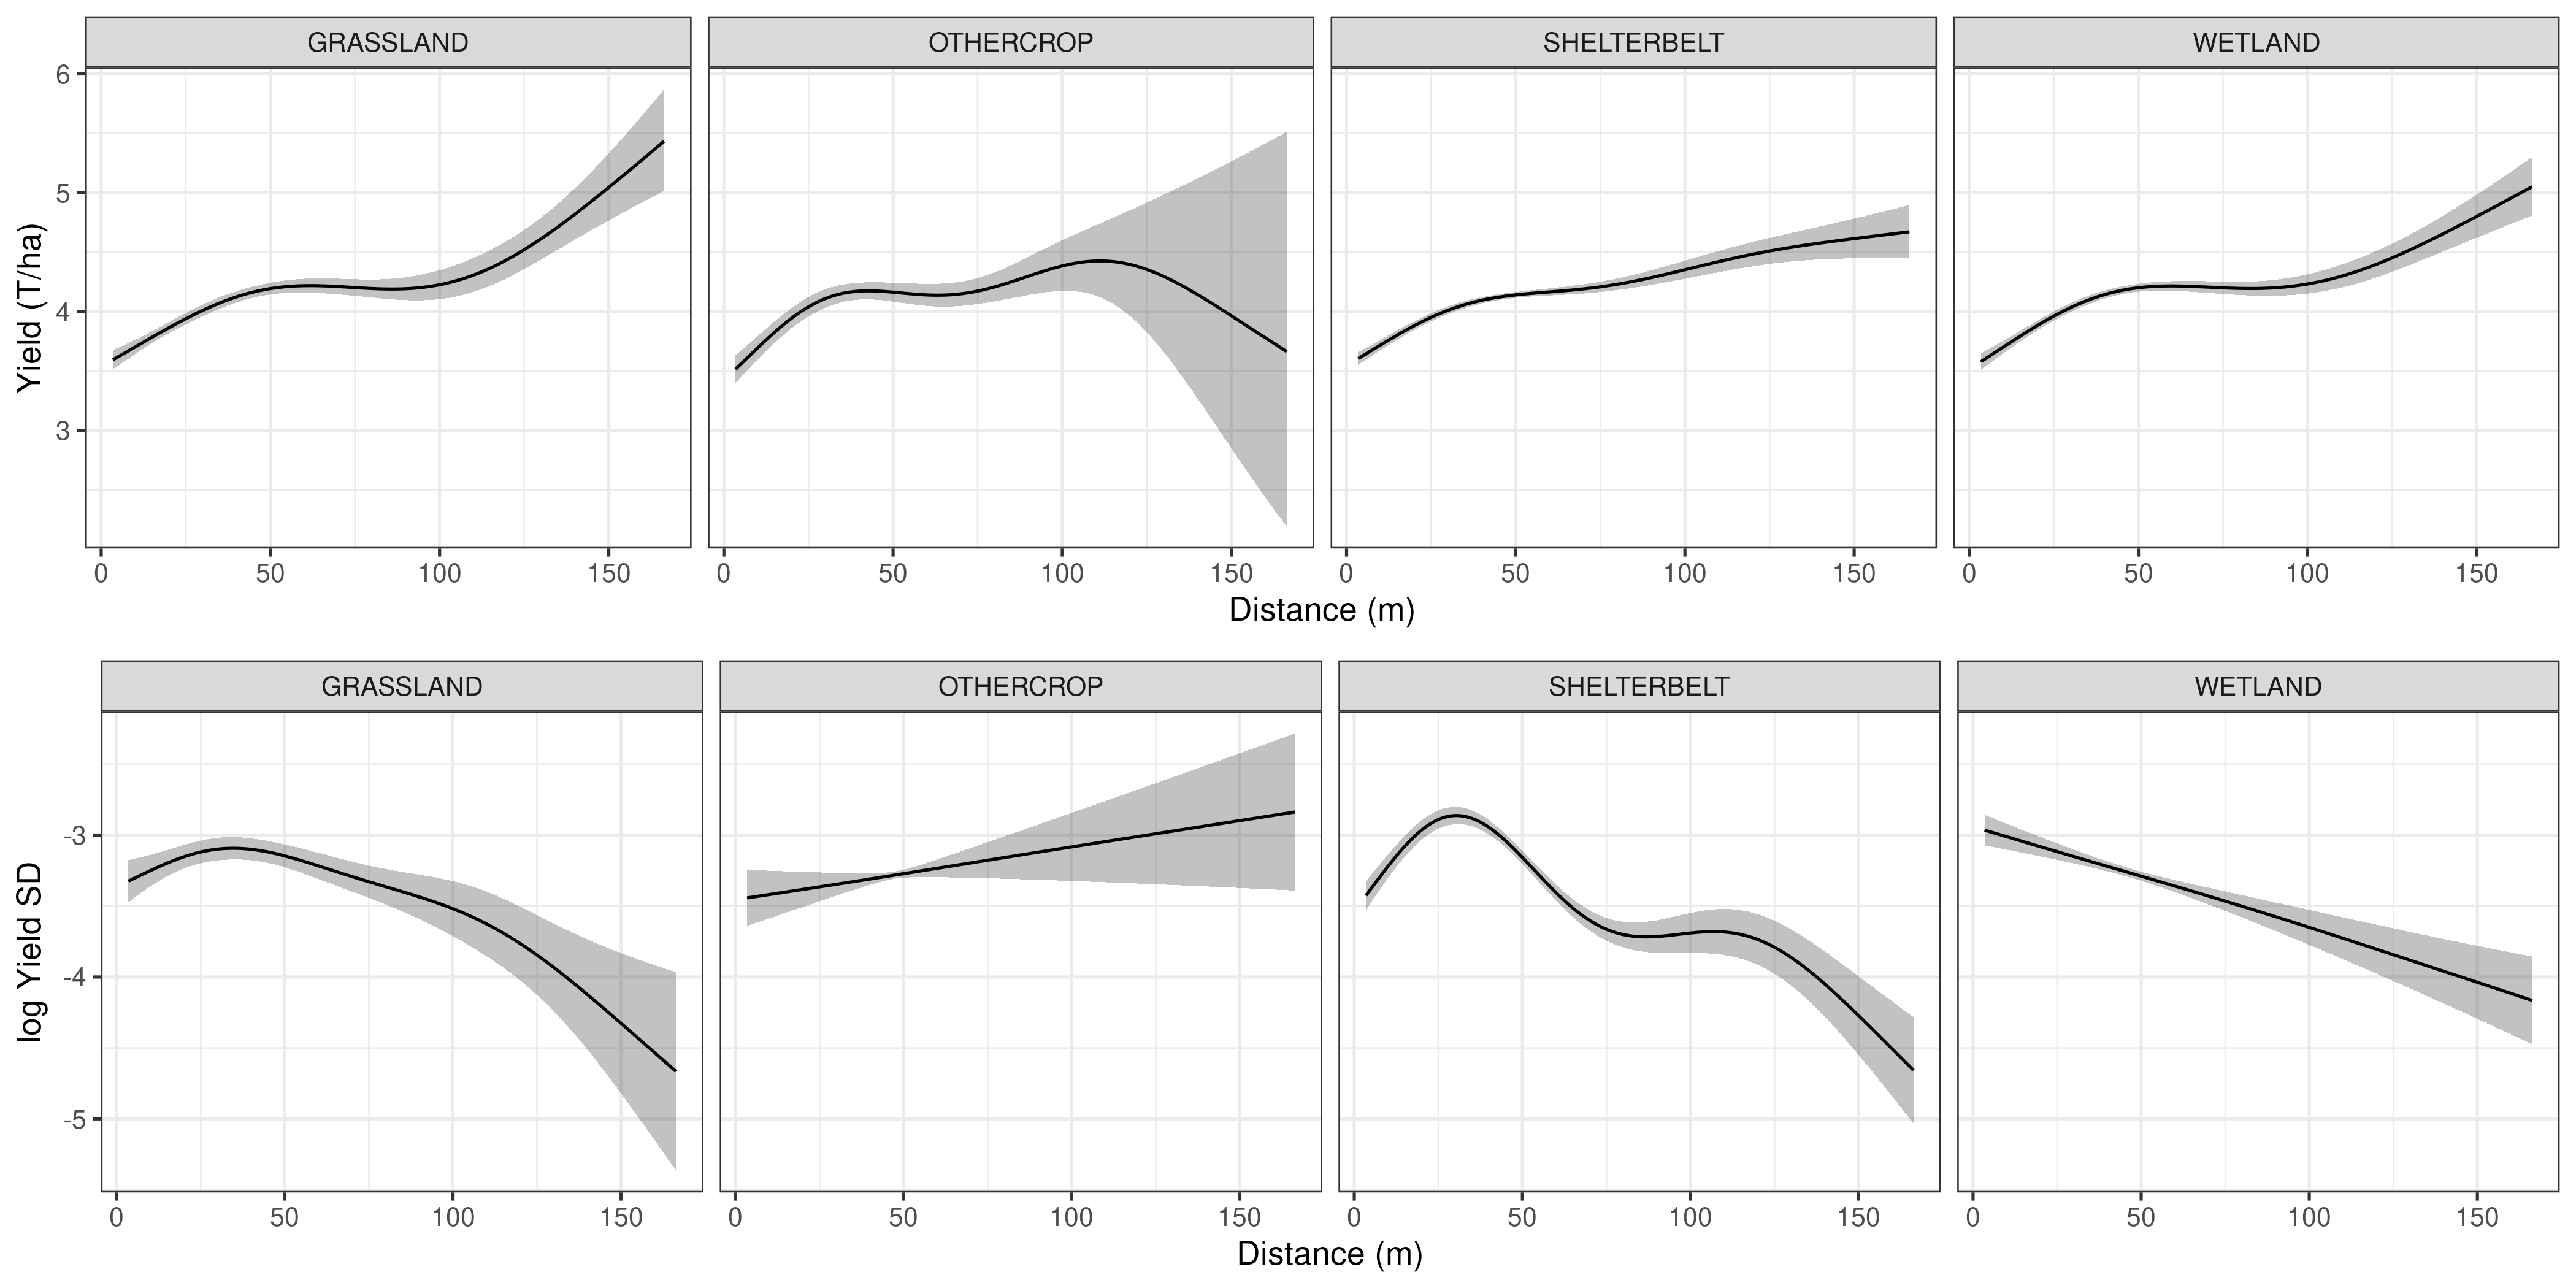
\includegraphics[width=1\linewidth]{../Figures/ExamplePlots/distSmooths} \caption{Distance smoothers from a single field.}\label{fig:distSmooths}
\end{figure}

\begin{figure}
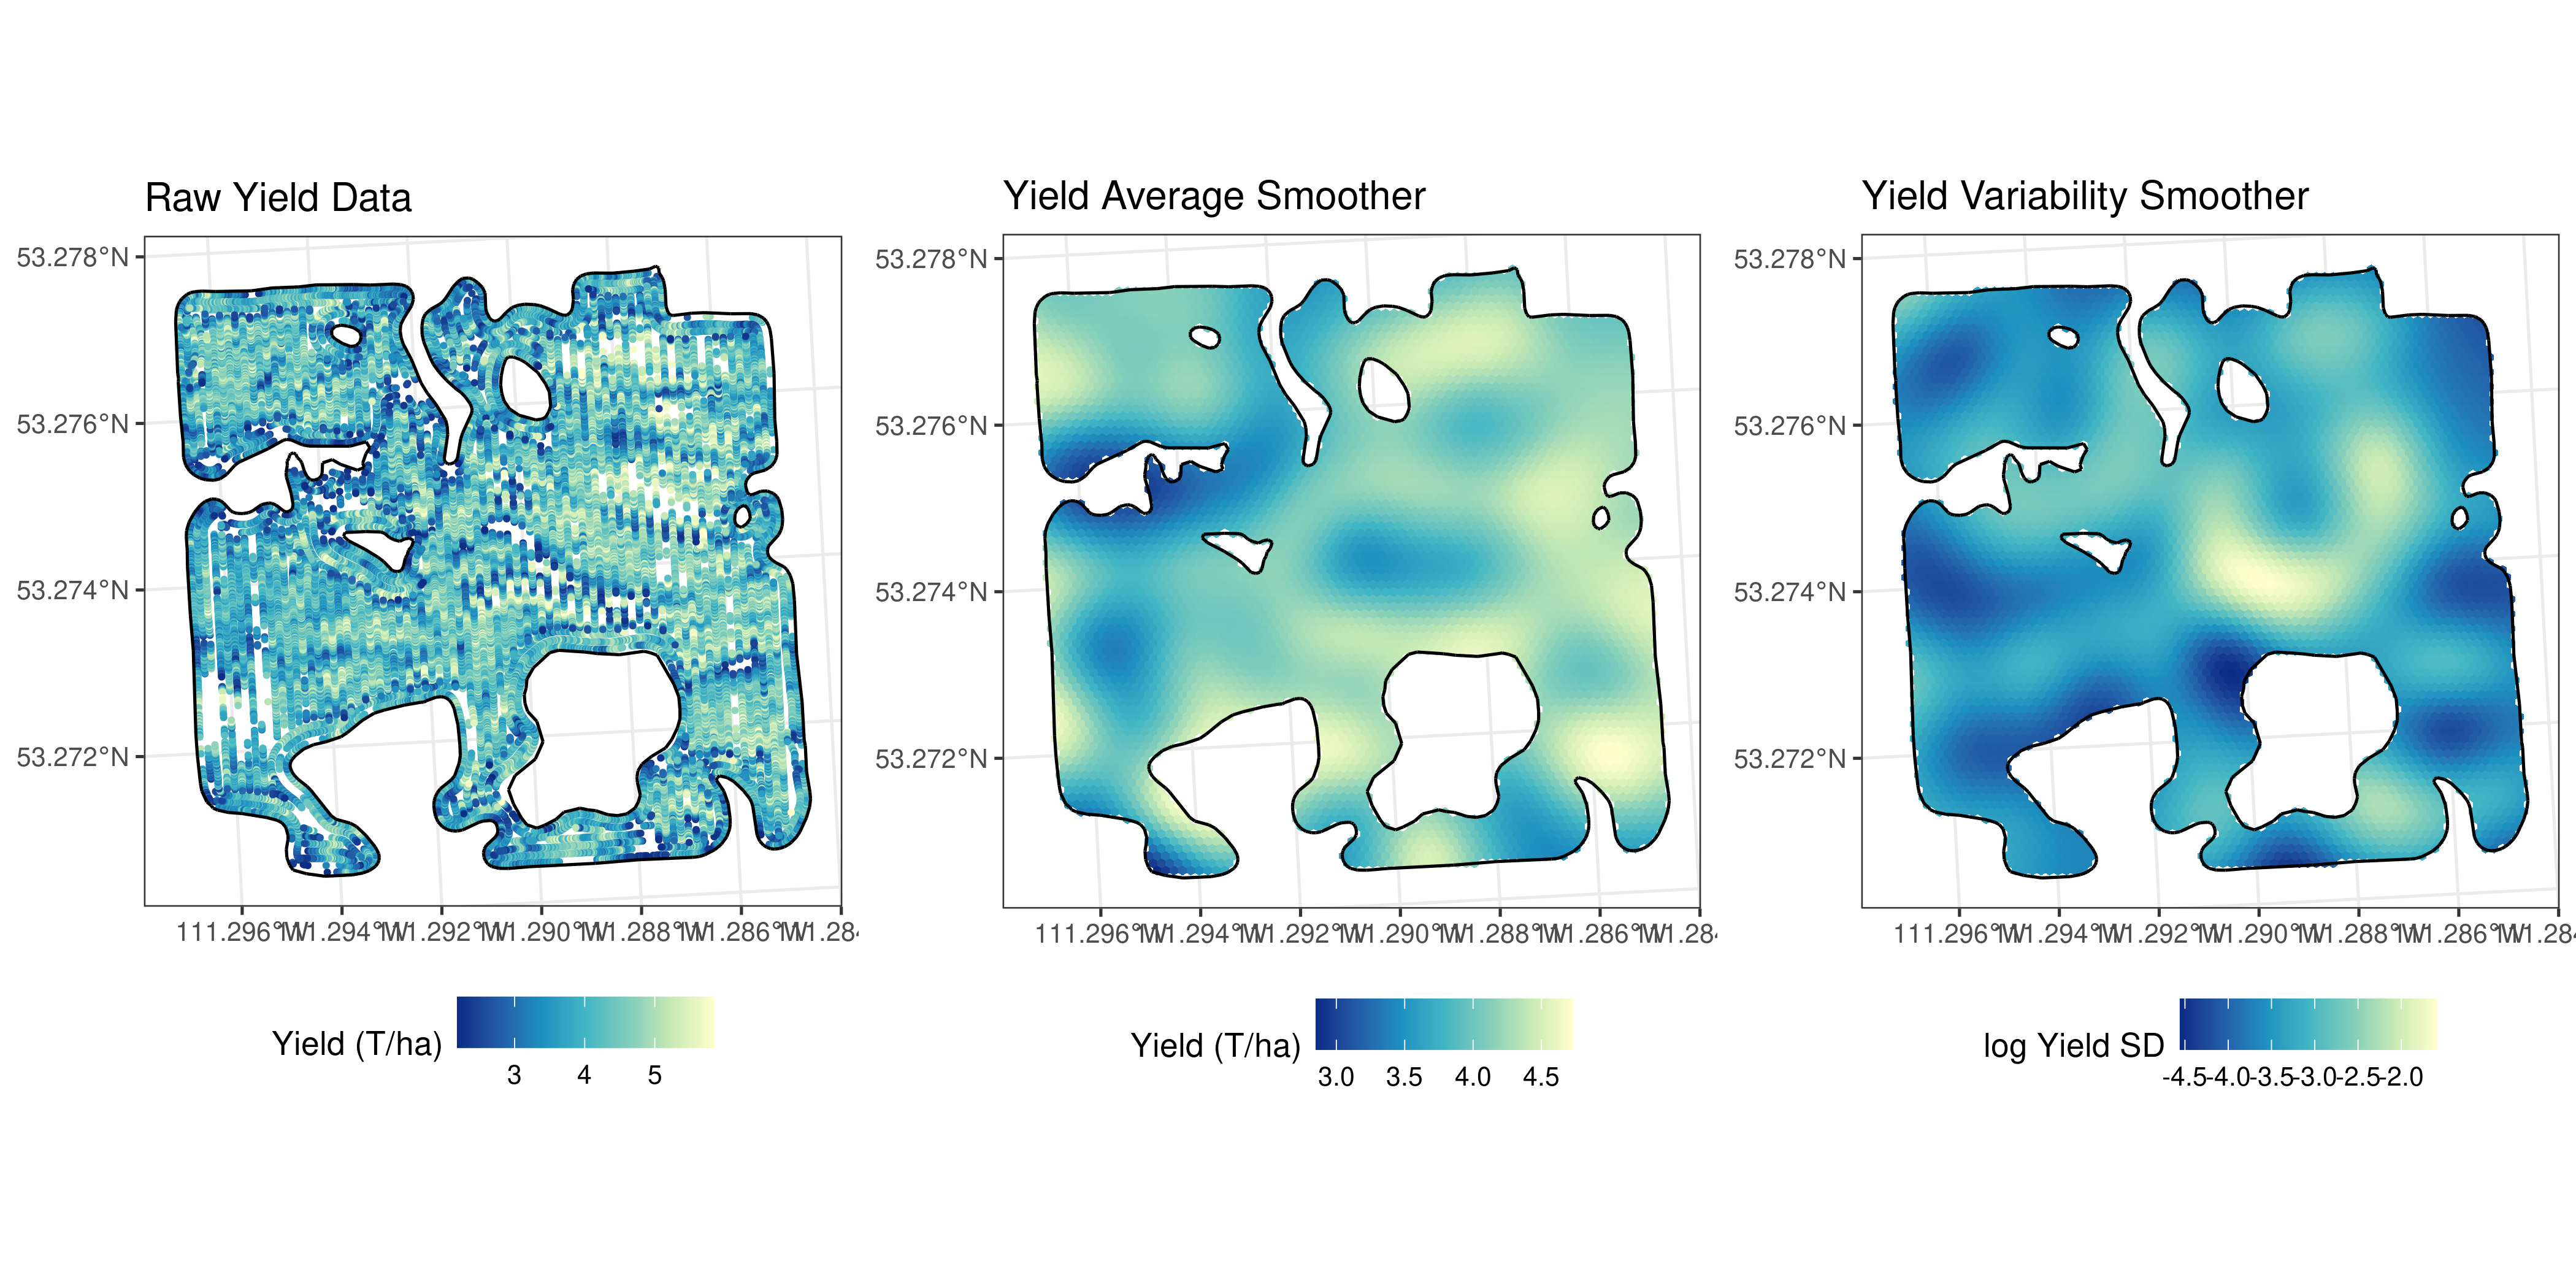
\includegraphics[width=1\linewidth]{../Figures/ExamplePlots/spatialSmooths} \caption{Spatial (random spatial variation) smoothers from a single field.}\label{fig:spatialSmooths}
\end{figure}

\hypertarget{overall-results}{%
\subsection{Overall results}\label{overall-results}}

Across all fields, Standard (grassy border) field boundaries were the most common boundary type, followed by Shelterbelts and Other Crops (Figure \ref{fig:boundaryTypes}).

\begin{figure}
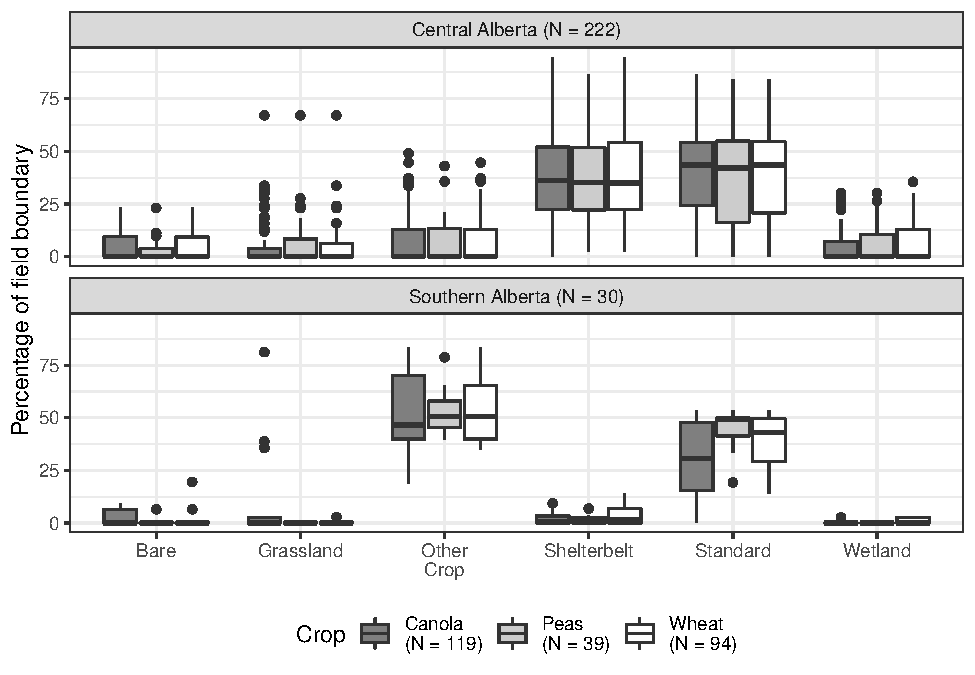
\includegraphics[width=1\linewidth]{manuscript_files/figure-latex/boundaryTypes-1} \caption{Percentage of field boundaries across sampled fields.}\label{fig:boundaryTypes}
\end{figure}

\hypertarget{canola-fields}{%
\subsubsection{Canola fields}\label{canola-fields}}

Overall, there was a strong negative effect of combine ground speed on both the average and variability of canola yield.
At the field level, both yield average and yield variability (SD of yield) of yield were extremely spatially (average p-values: 2e-16, 1.77e-05) and temporally dependent (2e-16, 0.000243), meaning that average and variability changed with location in the field, as well as sequentially during the harvest.
However, there was no difference in average or variability with harvest sequence when all fields were considered, meaning that combines did not appear to distort yield data from start to finish in any systematic way.

Average canola yield tended to increase with distance from Standard and Other Crop boundaries, leveling off at about 25 m (Figure \ref{fig:canolaPlot} top row, Other crop and Standard panels); yield was approximately 0.1 T/ha (1.5 bu/ac) lower at the edge for both of these boundary types.
Interestingly, Shelterbelts were well-represented in the data (Figure \ref{fig:boundaryTypes}) but the negative edge effect was not strong (Figure \ref{fig:canolaPlot} top row, Shelterbelt panel), indicating that they may provide better micro-climates for crops located near them.
Other boundary types were less common in the data and had correspondingly weaker effects on mean yield, but all showed a small negative edge effect.
Yield variability tended to decrease with distance from the edge of the field, indicating that edge effects contribute to yield ``patchiness'' as well as averages.
At Standard, Bare, and Wetland field boundaries, variability decreased until about 100 m, after which variability was constant, while the pattern was less consistent in Grassland, Other Crop, and Shelterbelt.

\begin{figure}
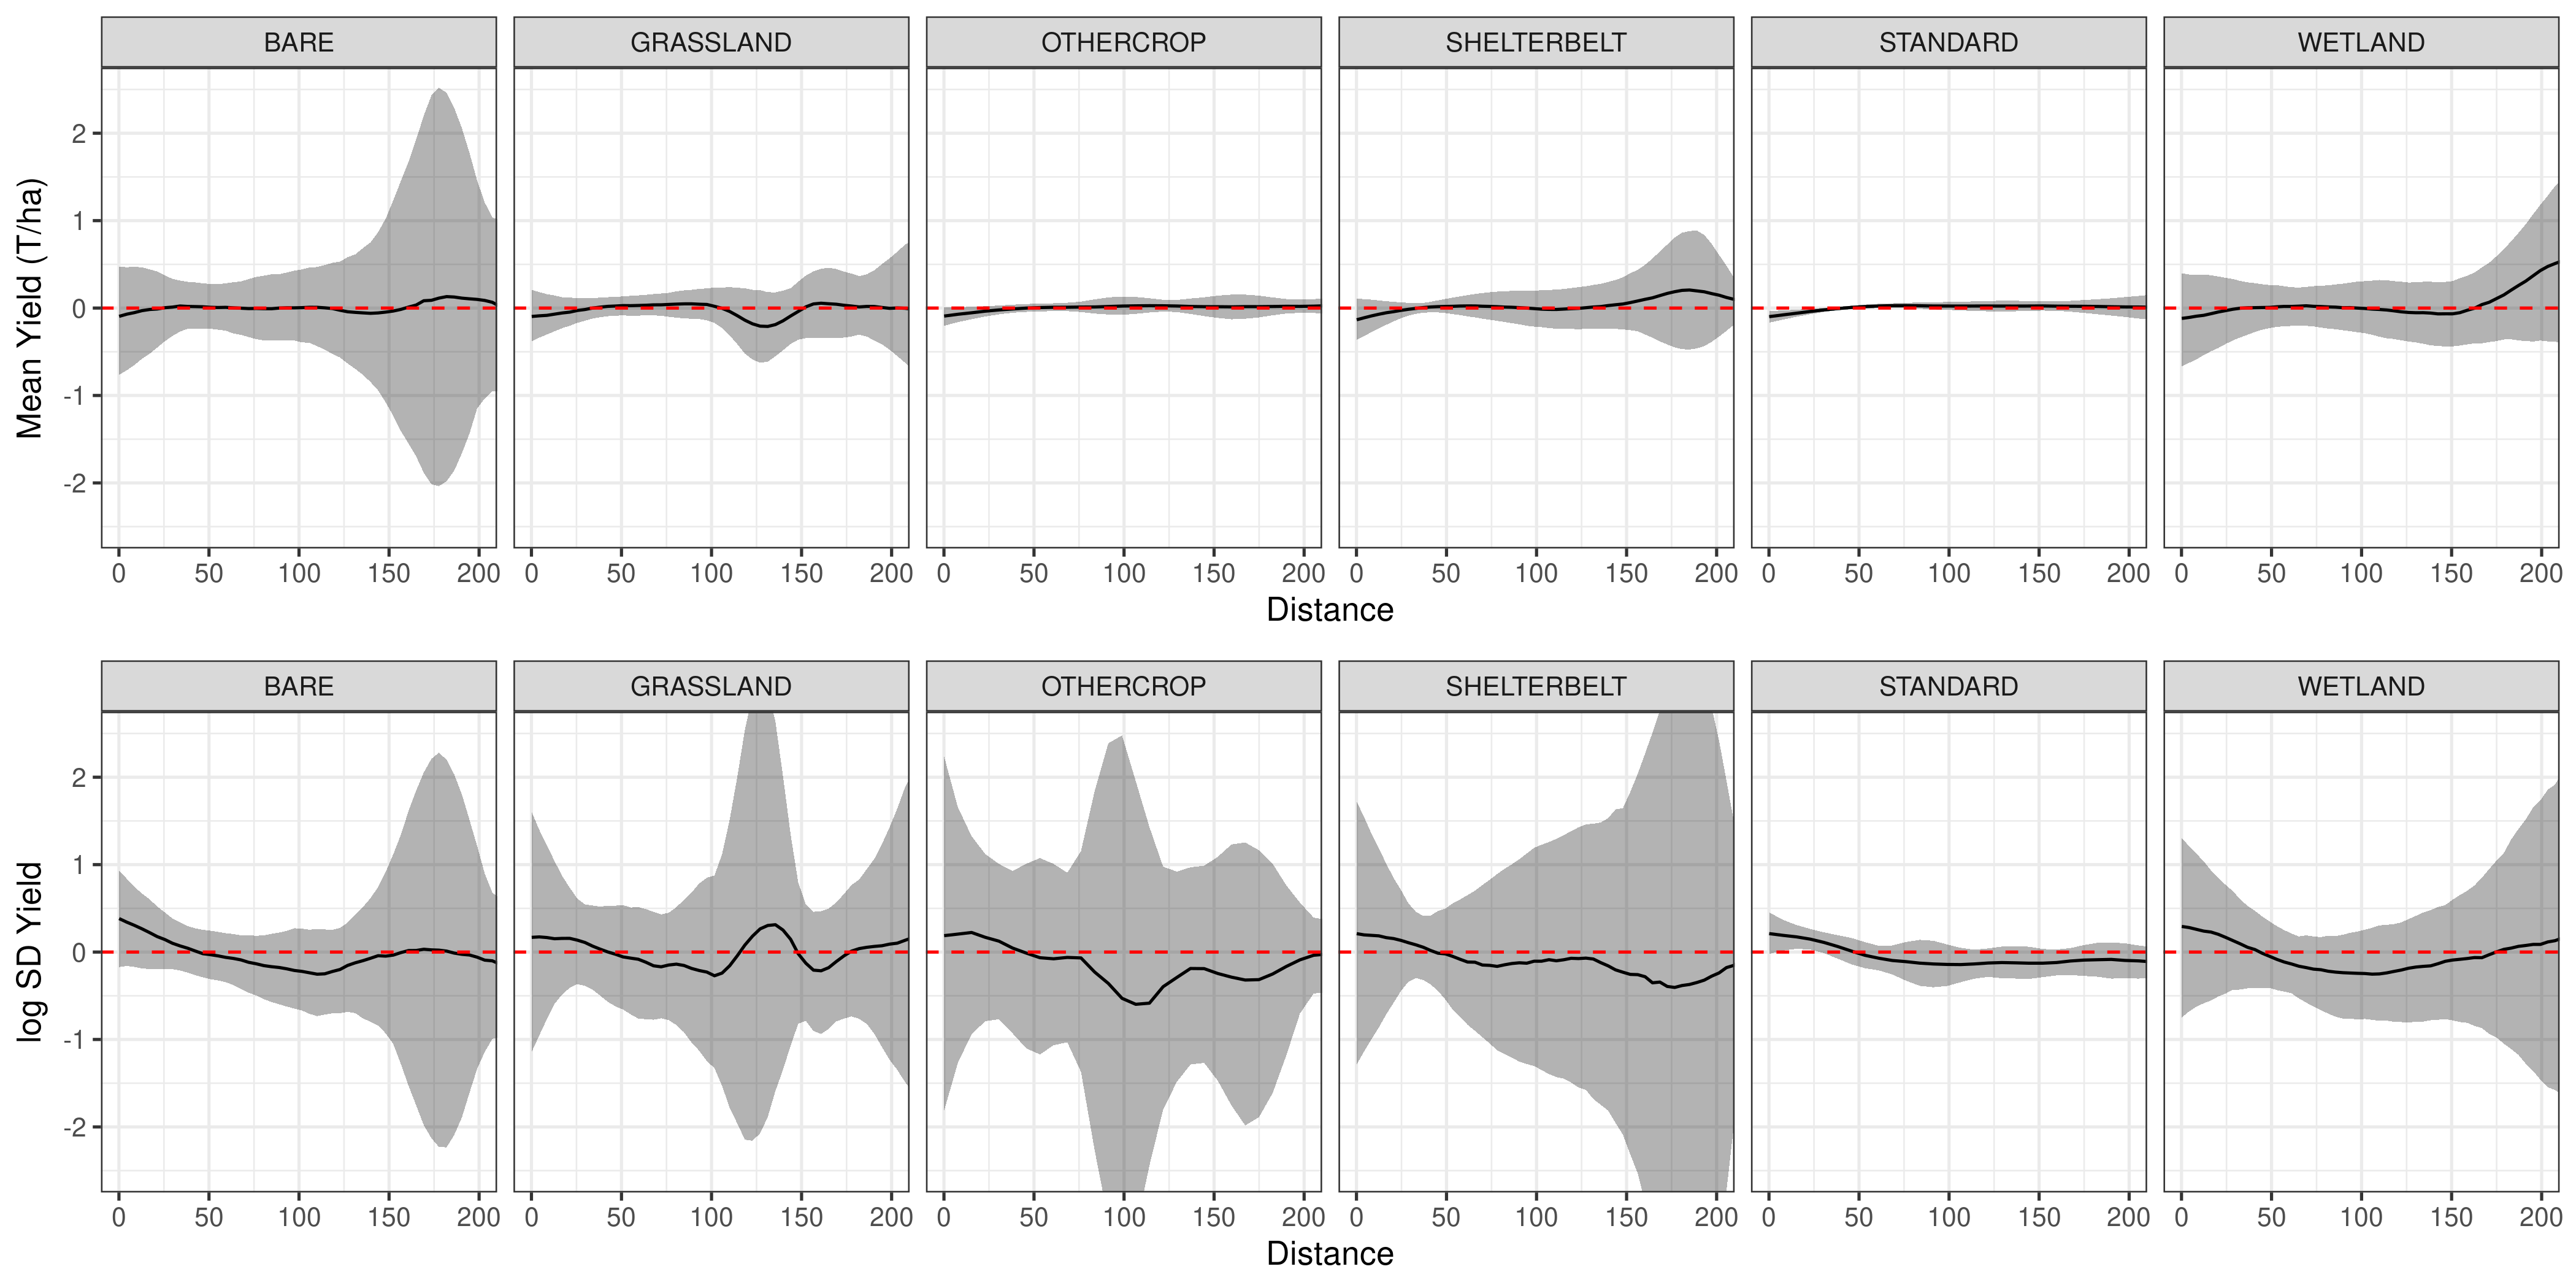
\includegraphics[width=1\linewidth]{../Figures/ModelSummary3a_canola} \caption{Field boundary effect on canola yield, accounting for the effect of combine speed, spatial variation, and harvest sequence. Upper panel represents mean yield, while the lower panel represents yield variation (i.e. "patchiness").}\label{fig:canolaPlot}
\end{figure}

\hypertarget{wheat-fields}{%
\subsubsection{Wheat fields}\label{wheat-fields}}

Similar to canola, there was a strong negative effect of ground speed on both yield and variability of wheat yield (Figure \ref{fig:wheatPlotSpeed}, left panels).
At the field level, both yield average and yield variability (SD of yield) of yield were spatially (average p-values: 2e-16, 2e-16) and temporally dependent (2e-16, 2e-16), but harvest sequence did not distort the average or SD of wheat yield in a systematic way (Figure \ref{fig:wheatPlotSpeed}, right panel).

Average wheat yield increased slightly with distance from the field boundary, but this was much more variable than the patterns seen in canola yield (Figure \ref{fig:wheatPlot}).
There was also a slight increase in variability away from the field boundary, at least for Standard and Other Crop boundaries, but this was inconsistent among other boundary types.

\begin{figure}
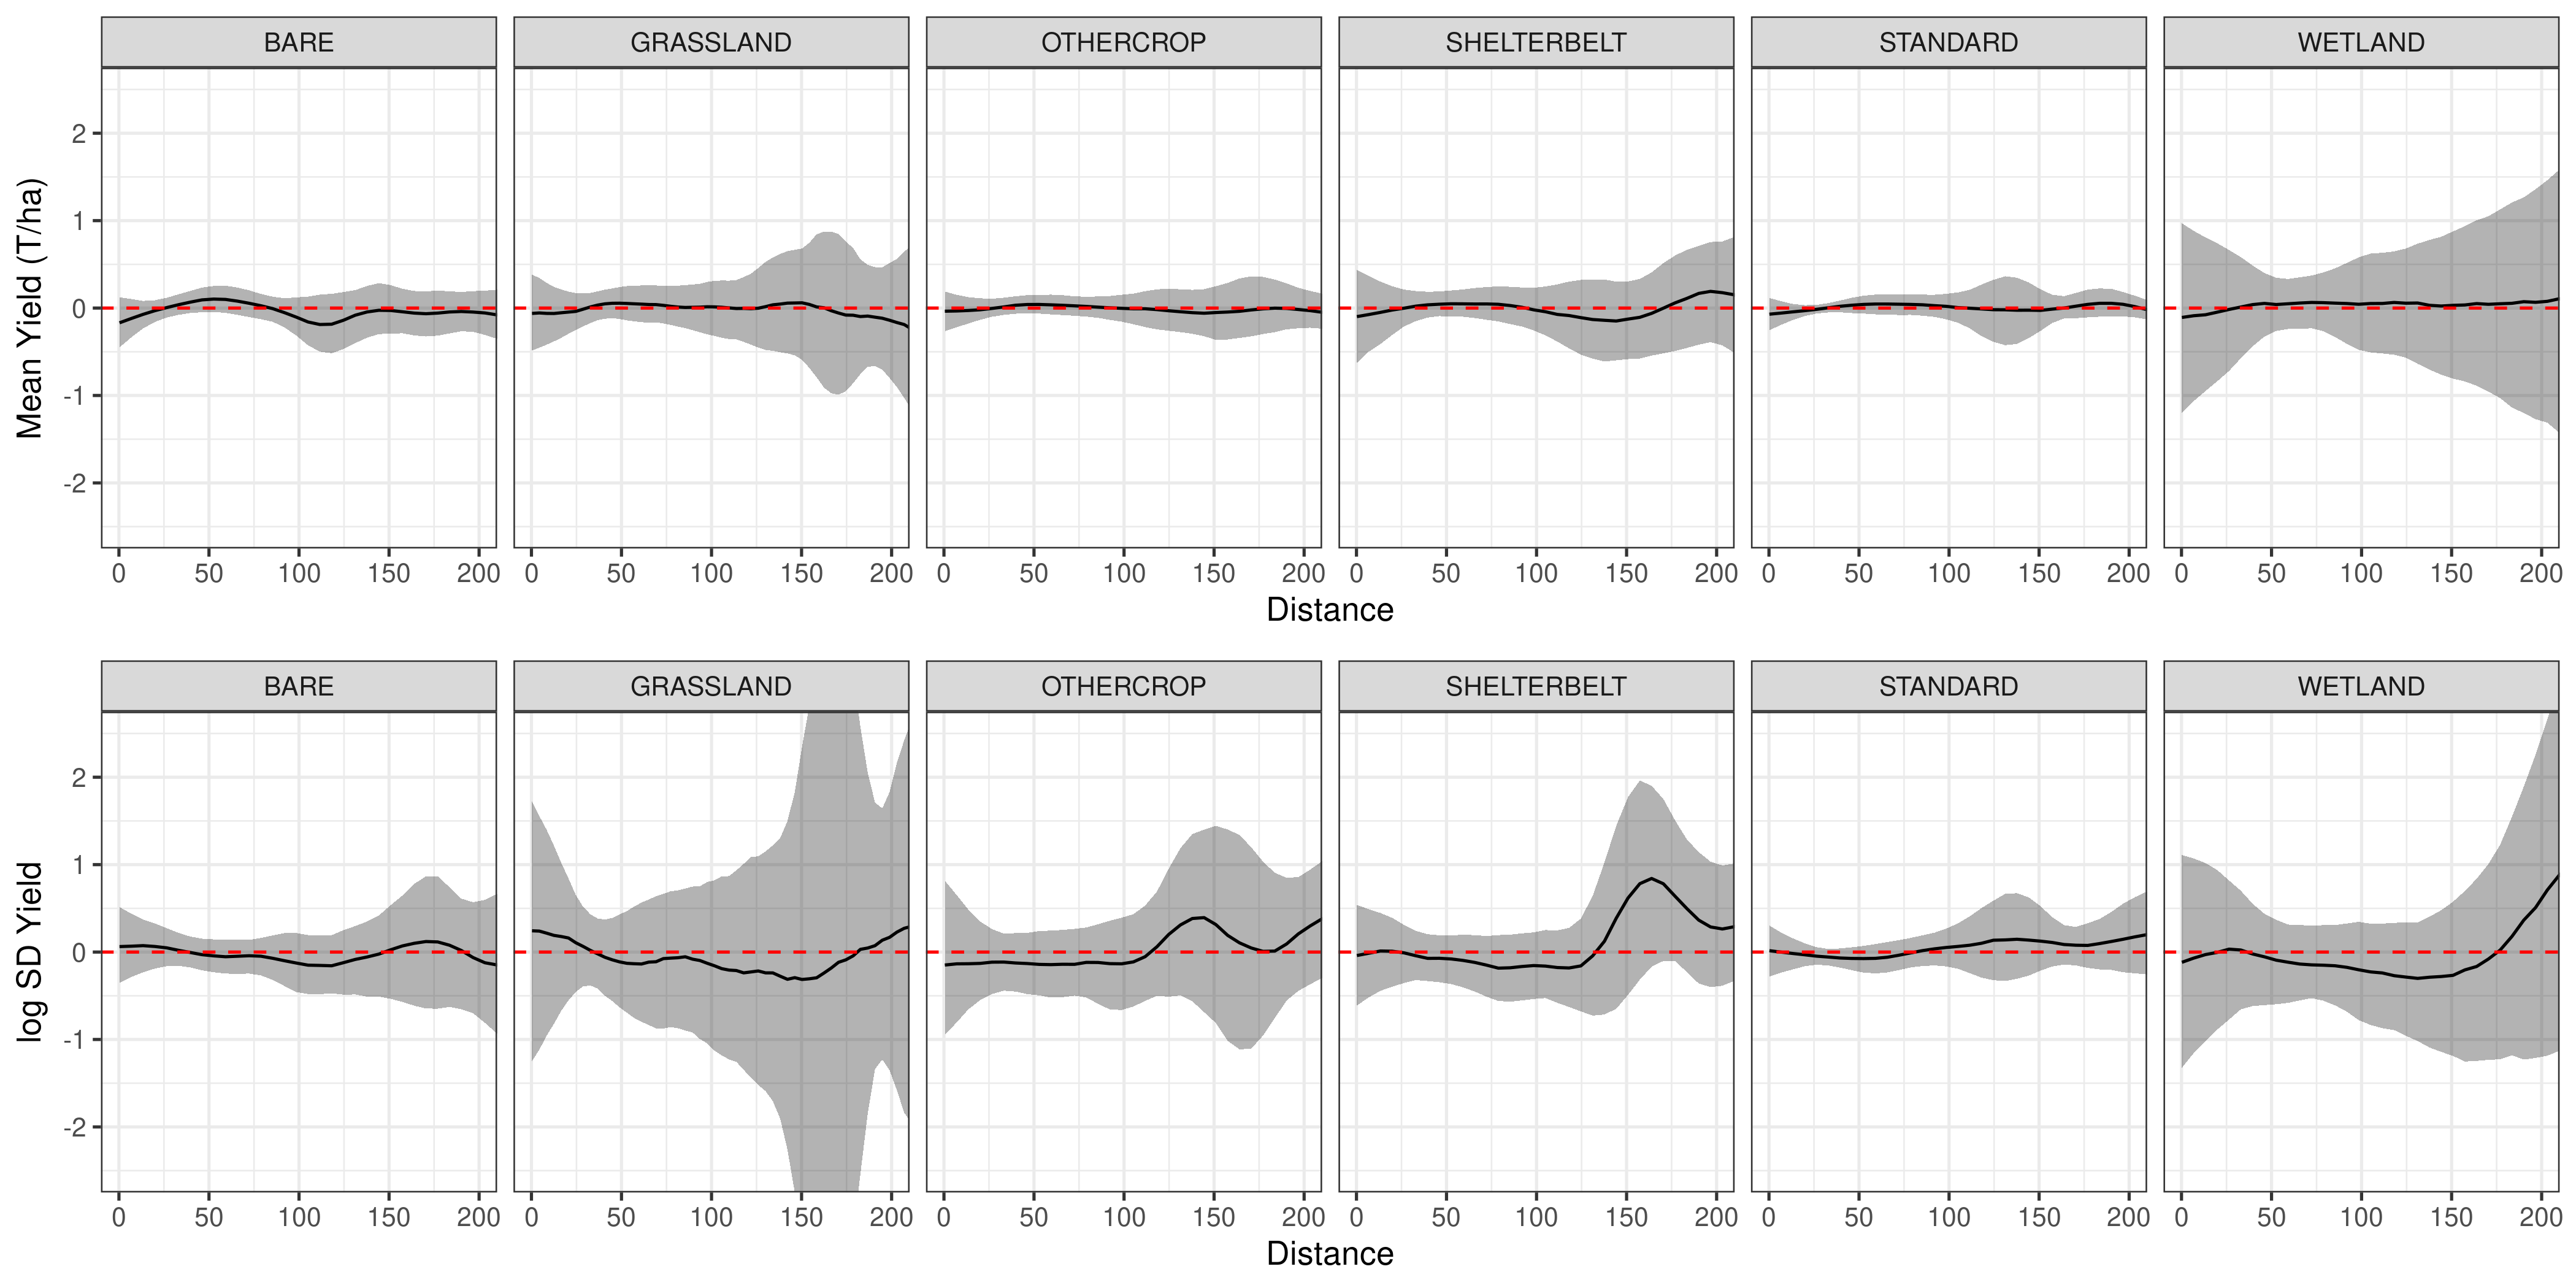
\includegraphics[width=1\linewidth]{../Figures/ModelSummary3a_wheat} \caption{Field boundary effect on canola yield, accounting for the effect of combine speed, spatial variation, and harvest sequence. Upper panel represents mean yield, while the lower panel represents yield variation (i.e. "patchiness").}\label{fig:wheatPlot}
\end{figure}

\hypertarget{pea-fields}{%
\subsubsection{Pea fields}\label{pea-fields}}

At the field level, both yield average and yield variability (SD of yield) of yield were spatially (average p-values: 2e-16, 2e-16) and temporally dependent (2e-16, 3.62e-07),
There was a strong negative effect of ground speed on yield and variability of peas (Figure \ref{fig:peasPlotSpeed}), but harvest sequence did not distort the average or SD of wheat yield in a systematic way (Figure \ref{fig:wheatPlotSpeed}, right panel).

Average pea yields increased with distance from Shelterbelt, Standard, and Wetland field boundaries.
Interestingly, the reduction at the edge was slightly higher for Wetlands, but yield increased with distance more quickly, i.e.~yields were higher at distance for Wetlands.
Variability decreased with distance from Grassland and Standard boundaries

\begin{figure}
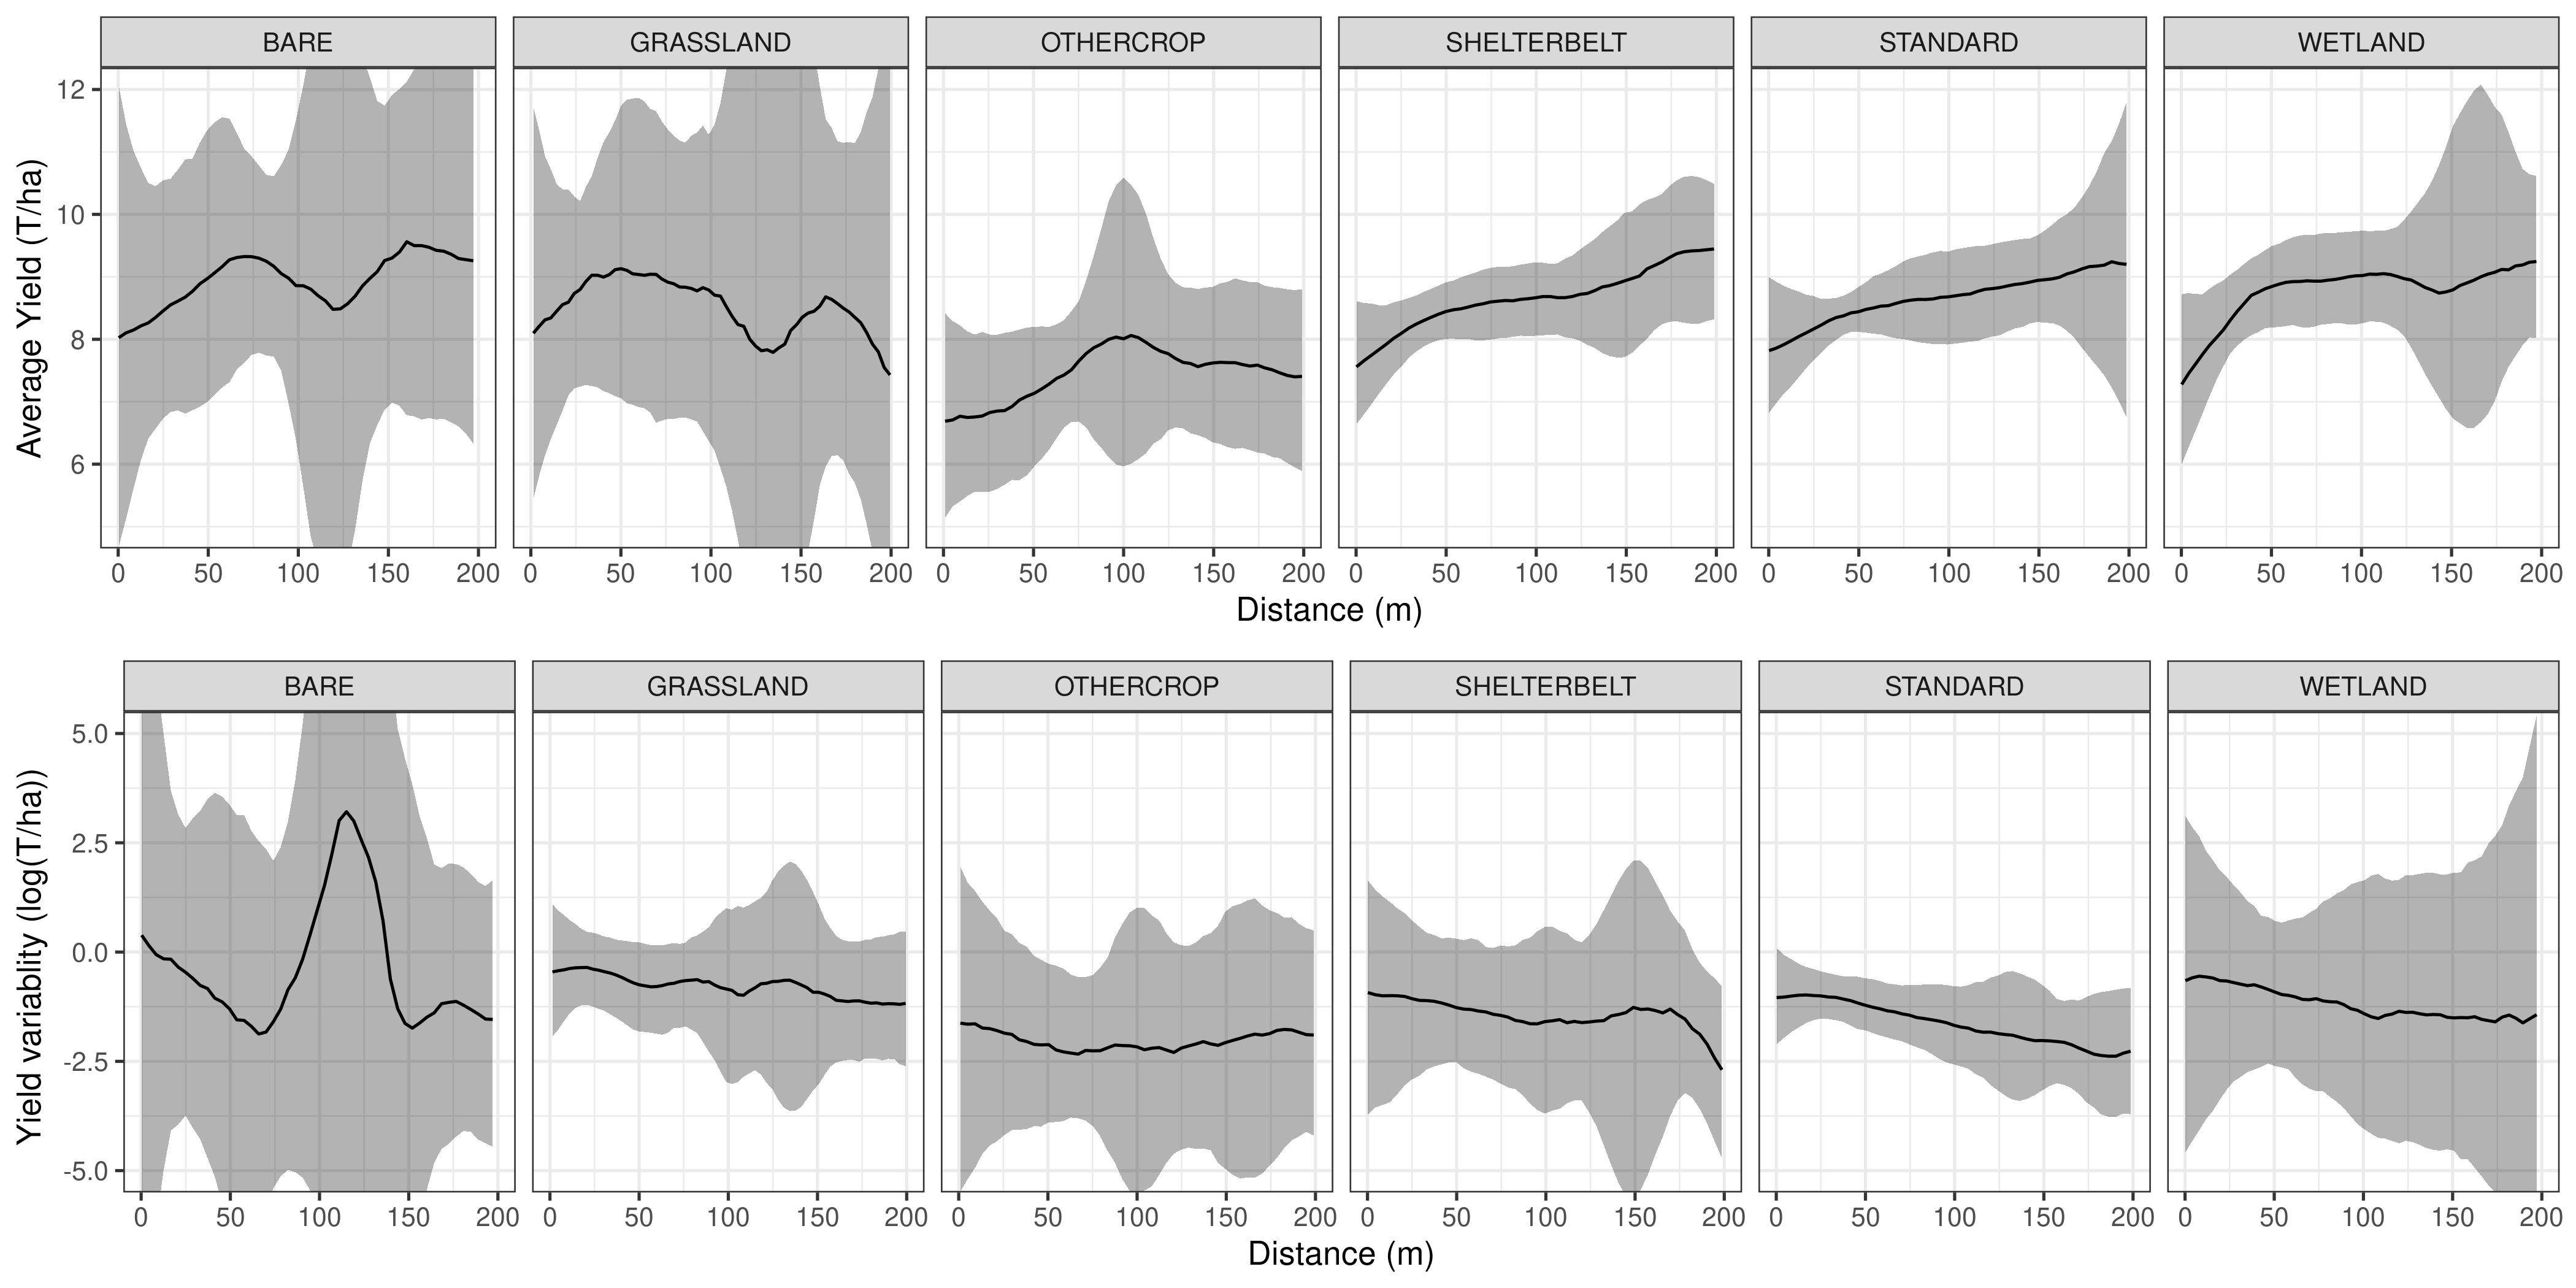
\includegraphics[width=1\linewidth]{../Figures/ModelSummary3a_peas} \caption{Field boundary effect on pea yield, accounting for the effect of combine speed, spatial variation, and harvest sequence. Upper panel represents mean yield, while the lower panel represents yield variation (i.e. "patchiness").}\label{fig:peaPlot}
\end{figure}

\hypertarget{discussion}{%
\section{Discussion}\label{discussion}}

At the level of individual fields, both average and SD of yield varied with distance from the field boundary.
Both metrics also varied with ground speed and harvest sequence, and there were strong spatial relationships within each field, likely related to underlying soil or moisture conditions.
Yield tended to increase with distance from field boundaries before plateauing, but there was little evidence of intermediate boosts in yield, meaning that ecosystem services likely increased or did not vary with distance from field boundaries (Scenario 2, Figure \ref{fig:hypotheses}).
Some crops displayed a larger decrease in yield next to field boundaries; for example, pea yield directly adjacent to Wetland was lower overall, but increased with distance more than other crop types, indicating that Wetlands may locally decrease pea yields but are beneficial to the crop in general.
Canola yields next to Other Crops had a reduced edge effect compared to Standard field boundaries, indicating that Other Crops may provide a more consistent microclimate for canola than grassy field boundaries.
However, the difference between boundary types tended to be both small and variable, especially for wheat.

Why did we find few consistent effects of boundary type on crop yield?
We consider a few potential reasons for this below:
1. Landscape influence
2. Boundary variables
3. Ecosystem disservices
4. Yearly/location variation
5. Lack of pest pressure/pollination deficit

Our analysis only examined boundary types, without considering the landscape context that fields were embedded in.
Some studies show the influence of landscape composition at larger spatial scales (e.g.~Lan's paper) which could be particularly important when beneficial arthropods are highly mobile (e.g.~bumblebee foraging) or disperse very broadly (Öberg \emph{et al.} 2007).
There could also be interactions between landscape composition at different scales (Motzke \emph{et al.} 2016; Robinson \emph{et al.} 2021), but this is not well-studied.
Landscape complexity (Fahrig \emph{et al.} 2011) and connectivity are also associated with higher abundance of beneficial arthropods (Paul's new paper + others).
This means that field boundaries such as wetlands or shelterbelts may only be helpful if connected to a larger network of non-crop habitat (but see Fahrig \emph{et al.} 2019).
Our definitions of boundary type were also (necessarily) loose, as we used satellite imagery to manually classify them.
However, it may be that other boundary traits, such as size or plant species composition, are more important for spillover of ecosystems services into fields.
For example, larger (Lecq \emph{et al.} 2018; Stašiov \emph{et al.} 2020) or more functionally diverse (Bonifacio \emph{et al.} 2011; Boughey \emph{et al.} 2011) hedgerows tend to support more biodiversity than smaller hedgerows, and some studies have shown that leaf litter and soil compaction matters to predatory beetle communities (Sutter \emph{et al.} 2018).
These fine-scale boundary characteristics were not measured in our study, but could be used as variables in more biologically-meaningful classifications of field boundaries.

Our first scenario (Scenario 1, Figure \ref{fig:hypotheses}) assumes that beneficial organisms disperse from boundaries into the field, and had a generally positive effect on crop yield.
However, field boundaries may not have a positive effect if a) pests (ecosystem dis-services) also disperse along with beneficials, b) if beneficials do not disperse from the boundary environment, or if c) the effect of beneficial organisms is small.
Ecosystem disservices such as pests and weeds can also disperse from field boundaries, which may negate any positive effect of ecosystem services (Zhang \emph{et al.} 2007).
Gray \& Lewis (2014) showed that remnant forest fragments do not provide significant pest control services , but also do not depress yield.
However, this is still poorly studied, and parsing out services from disservices is impossible using crop yield data \emph{alone}.
Ecosystem services from field boundaries may be limited if beneficial organisms stay in field boundaries, or disperse at wider spatial scales Robinson \emph{et al.} (2021).
Finally, pest pressure or pollination deficit may be low enough that ecosystem service provision does not significantly change yield.
Canola is largely self-pollinating (at least in hybrid canola varieties, Lindström \emph{et al.} 2016) and wheat is wind-pollinated, meaning that slight increases in pollination services may not change yields significantly in either crop (Woodcock \emph{et al.} 2016).
Pests are also limited by growers' application of insecticides (seed-treated or on the crop directly), and insect pest outbreaks tend to be temporally and spatially spotty.

Since our sampling represents a limited amount of spatial and temporal coverage, there could be additional confounding variables that obscure signals of yield.
Most fields were located in Central Alberta (Dry Mixedwood region, Natural Regions Committee 2006), where boundaries contained a higher proportion of Shelterbelts (Figure \ref{fig:boundaryTypes}), but differences from Southern AB (Foothills Fescue and Mixedgrass region) may be confounding the signal.
Between-year effects may be important, especially during dry years (Kort 1988), but this was not considered in our analysis.
Future work could examine whether boundaries have differing effects during hot or cool years.

We used harvest time as smoothed variable to deal with temporal autocorrelation in the data, but this is a crude way to deal with this.
This is because in-field combine driving patterns \emph{almost always} induce correlation between spatial and temporal measurements (e.g.~northern section of the field was harvested before the southern section), meaning that temporal and spatial random effects are difficult to separate.
There are few solutions to this using harvest data as-is, other than to ignore temporal random effects entirely, thereby constraining all random variation to be spatial.
However, it is possible to remove correlation between spatial and temporal measurements by using specially designed harvest patterns within a field (harvesting alternating strips sequentially across the field, then harvesting the remaining strips on a second pass).
Future studies could use this to estimate drift in combine sensor measurements over time.

\hypertarget{author-contributions}{%
\section{Author Contributions}\label{author-contributions}}

SVJR and PG conceived of the project.
SVJR collected data, conducted analysis, and wrote the manuscript.

\hypertarget{acknowledgements}{%
\section{Acknowledgements}\label{acknowledgements}}

We thank Trent Clark, Dean Hubbard, Alvin French, and Kristina Polziehn for providing yield data for us, and providing insight on their yield data.
We also thank Autumn Barnes and Keith Gabert of the Canola Council of Canada, and Laurel Thompson and JP Pettyjohn of Lakeland College for connecting us with farmers and agronomists.
Funding for this research was provided by Ducks Unlimited Canada's Institute for Wetland and Waterfowl Research, the Alberta Canola Producers Commission, Manitoba Canola Growers Association, SaskCanola, the Alberta Biodiversity Monitoring Institute, and the Alberta Conservation Association.

\hypertarget{references}{%
\section*{References}\label{references}}
\addcontentsline{toc}{section}{References}

\hypertarget{refs}{}
\begin{CSLReferences}{1}{0}
\leavevmode\hypertarget{ref-albrecht2020}{}%
Albrecht, M., Kleijn, D., Williams, N.M., Tschumi, M., Blaauw, B.R., Bommarco, R., \emph{et al.} (2020). The effectiveness of flower strips and hedgerows on pest control, pollination services and crop yield: A quantitative synthesis. \emph{Ecology Letters}.

\leavevmode\hypertarget{ref-arslan2002}{}%
Arslan, S. \& Colvin, T.S. (2002). An evaluation of the response of yield monitors and combines to varying yields. \emph{Precision Agriculture}, 3, 107--122.

\leavevmode\hypertarget{ref-baker2018}{}%
Baker, T.P., Moroni, M.T., Mendham, D.S., Smith, R. \& Hunt, M.A. (2018). Impacts of windbreak shelter on crop and livestock production. \emph{Crop and Pasture Science}, 69, 785.

\leavevmode\hypertarget{ref-bonifacio2011}{}%
Bonifacio, R.S., Kinross, C.M., Gurr, G.M. \& Nicol, H. (2011). The effect of woody plant diversity and other stand and landscape factors on the diversity and abundance of birds using farm shelterbelts. \emph{Pacific Conservation Biology}, 17, 22.

\leavevmode\hypertarget{ref-boughey2011}{}%
Boughey, K.L., Lake, I.R., Haysom, K.A. \& Dolman, P.M. (2011). Improving the biodiversity benefits of hedgerows: How physical characteristics and the proximity of foraging habitat affect the use of linear features by bats. \emph{Biological Conservation}, 144, 1790--1798.

\leavevmode\hypertarget{ref-brandle2004}{}%
Brandle, J.R., Hodges, L. \& Zhou, X.H. (2004). Windbreaks in {North American} agricultural systems. In: \emph{New vistas in agroforestry: A compendium for 1st world congress of agroforestry, 2004} (eds. Nair, P.K.R., Rao, M.R. \& Buck, L.E.). Springer Netherlands, Dordrecht, pp. 65--78.

\leavevmode\hypertarget{ref-case2019}{}%
Case, B.S., Pannell, J.L., Stanley, M.C., Norton, D.A., Brugman, A., Funaki, M., \emph{et al.} (2019). Non-production vegetation has a positive effect on ecological processes in agroecosystems. \emph{bioRxiv}, 624635.

\leavevmode\hypertarget{ref-fahrig2019}{}%
Fahrig, L., Arroyo-Rodríguez, V., Bennett, J.R., Boucher-Lalonde, V., Cazetta, E., Currie, D.J., \emph{et al.} (2019). Is habitat fragmentation bad for biodiversity? \emph{Biological Conservation}, 230, 179--186.

\leavevmode\hypertarget{ref-fahrig2011}{}%
Fahrig, L., Baudry, J., Brotons, L., Burel, F.G., Crist, T.O., Fuller, R.J., \emph{et al.} (2011). Functional landscape heterogeneity and animal biodiversity in agricultural landscapes. \emph{Ecology Letters}, 14, 101--112.

\leavevmode\hypertarget{ref-gardner2021}{}%
Gardner, E., Breeze, T.D., Clough, Y., Smith, H.G., Baldock, K.C.R., Campbell, A., \emph{et al.} (2021). Field boundary features can stabilise bee populations and the pollination of mass-flowering crops in rotational systems. \emph{Journal of Applied Ecology}, In press.

\leavevmode\hypertarget{ref-garibaldi2011}{}%
Garibaldi, L.A., Steffan-Dewenter, I., Kremen, C., Morales, J.M., Bommarco, R., Cunningham, S.A., \emph{et al.} (2011). Stability of pollination services decreases with isolation from natural areas despite honey bee visits. \emph{Ecology Letters}, 14, 1062--1072.

\leavevmode\hypertarget{ref-gray2014}{}%
Gray, C.L. \& Lewis, O.T. (2014). Do riparian forest fragments provide ecosystem services or disservices in surrounding oil palm plantations? \emph{Basic and Applied Ecology}, 15, 693--700.

\leavevmode\hypertarget{ref-kassambara2020}{}%
Kassambara, A. (2020). \emph{{ggpubr}: 'ggplot2' based publication ready plots}.

\leavevmode\hypertarget{ref-kort1988}{}%
Kort, J. (1988). 9. Benefits of windbreaks to field and forage crops. \emph{Agriculture, Ecosystems {\&} Environment}, 22-23, 165--190.

\leavevmode\hypertarget{ref-kowalchuk1995}{}%
Kowalchuk, T.E. \& Jong, E. de. (1995). Shelterbelts and their effect on crop yield. \emph{Canadian Journal of Soil Science}, 75, 543--550.

\leavevmode\hypertarget{ref-lecq2018}{}%
Lecq, S., Loisel, A., Mullin, S.J. \& Bonnet, X. (2018). Manipulating hedgerow quality: Embankment size influences animal biodiversity in a peri-urban context. \emph{Urban Forestry {\&} Urban Greening}, 35, 1--7.

\leavevmode\hypertarget{ref-lindstrom2016}{}%
Lindström, S.A.M., Herbertsson, L., Rundlöf, M., Smith, H.G. \& Bommarco, R. (2016). Large-scale pollination experiment demonstrates the importance of insect pollination in winter oilseed rape. \emph{Oecologia}, 180, 759--769.

\leavevmode\hypertarget{ref-lowe2021}{}%
Lowe, E.B., Groves, R. \& Gratton, C. (2021). Impacts of field-edge flower plantings on pollinator conservation and ecosystem service delivery {{}} a meta-analysis. \emph{Agriculture, Ecosystems {\&} Environment}, 310, 107290.

\leavevmode\hypertarget{ref-motzke2016}{}%
Motzke, I., Klein, A.-M., Saleh, S., Wanger, T.C. \& Tscharntke, T. (2016). Habitat management on multiple spatial scales can enhance bee pollination and crop yield in tropical homegardens. \emph{Agriculture, Ecosystems \& Environment}, 223, 144--151.

\leavevmode\hypertarget{ref-ABRegions2006}{}%
Natural Regions Committee. (2006). \emph{Natural regions and subregions of {Alberta}}. Government of Alberta, Edmonton.

\leavevmode\hypertarget{ref-oberg2007}{}%
Öberg, S., Ekbom, B. \& Bommarco, R. (2007). Influence of habitat type and surrounding landscape on spider diversity in {Swedish} agroecosystems. \emph{Agriculture, Ecosystems {\&} Environment}, 122, 211--219.

\leavevmode\hypertarget{ref-prietoBenitez2011}{}%
Prieto-Benítez, S. \& Méndez, M. (2011). Effects of land management on the abundance and richness of spiders ({Araneae}): A meta-analysis. \emph{Biological Conservation}, 144, 683--691.

\leavevmode\hypertarget{ref-quinn2017}{}%
Quinn, N.F., Brainard, D.C. \& Szendrei, Z. (2017). Floral strips attract beneficial insects but do not enhance yield in cucumber fields. \emph{Journal of Economic Entomology}, 110, 517--524.

\leavevmode\hypertarget{ref-redhead2020}{}%
Redhead, J.W., Oliver, T.H., Woodcock, B.A. \& Pywell, R.F. (2020). The influence of landscape composition and configuration on crop yield resilience. \emph{Journal of Applied Ecology}, 57, 2180--2190.

\leavevmode\hypertarget{ref-robinson2021}{}%
Robinson, S.V.J., Edwards, D., Vickruck, J.L., Best, L.R. \& Galpern, P. (2021). Non-crop sources of beneficial arthropods vary within-season across a prairie agroecosystem. \emph{Agriculture, Ecosystems {\&} Environment}, 320, 107581.

\leavevmode\hypertarget{ref-stasiov2020}{}%
Stašiov, S., Diviaková, A., Svitok, M., Novikmec, M. \& Dovciak, M. (2020). Hedgerows support rich communities of harvestmen ({Opiliones}) in upland agricultural landscape. \emph{Basic and Applied Ecology}, 47, 73--82.

\leavevmode\hypertarget{ref-sutter2018b}{}%
Sutter, L., Amato, M., Jeanneret, P. \& Albrecht, M. (2018). Overwintering of pollen beetles and their predators in oilseed rape and semi-natural habitats. \emph{Agriculture, Ecosystems {\&} Environment}, 265, 275--281.

\leavevmode\hypertarget{ref-vanVooren2017}{}%
Van Vooren, L., Bert, R., Steven, B., Pieter, D.F., Victoria, N., Paul, P., \emph{et al.} (2017). Ecosystem service delivery of agri-environment measures: A synthesis for hedgerows and grass strips on arable land. \emph{Agriculture, Ecosystems {\&} Environment}, 244, 32--51.

\leavevmode\hypertarget{ref-weninger2021}{}%
Weninger, T., Scheper, S., Lackóová, L., Kitzler, B., Gartner, K., King, N.W., \emph{et al.} (2021). Ecosystem services of tree windbreaks in rural landscapes -- a systematic review. \emph{Environmental Research Letters}, In press.

\leavevmode\hypertarget{ref-wickham2016}{}%
Wickham, H. (2016). \emph{{ggplot2}: Elegant graphics for data analysis}. Springer-Verlag New York.

\leavevmode\hypertarget{ref-wood2017}{}%
Wood, S.N. (2017). \emph{Generalized additive models: An introduction with {R}}. CRC press.

\leavevmode\hypertarget{ref-woodcock2016}{}%
Woodcock, B.A., Bullock, J.M., McCracken, M., Chapman, R.E., Ball, S.L., Edwards, M.E., \emph{et al.} (2016). Spill-over of pest control and pollination services into arable crops. \emph{Agriculture, Ecosystems \& Environment}, 231, 15--23.

\leavevmode\hypertarget{ref-zamorano2020}{}%
Zamorano, J., Bartomeus, I., Grez, A.A. \& Garibaldi, L.A. (2020). Field margin floral enhancements increase pollinator diversity at the field edge but show no consistent spillover into the crop field: A meta-analysis. \emph{Insect Conservation and Diversity}, 13, 519--531.

\leavevmode\hypertarget{ref-zhang2007}{}%
Zhang, W., Ricketts, T.H., Kremen, C., Carney, K. \& Swinton, S.M. (2007). Ecosystem services and dis-services to agriculture. \emph{Ecological Economics}, 64, 253--260.

\end{CSLReferences}

\newpage

\hypertarget{appendix-a-supplementary-material}{%
\section*{Appendix A: Supplementary Material}\label{appendix-a-supplementary-material}}
\addcontentsline{toc}{section}{Appendix A: Supplementary Material}

\begin{figure}
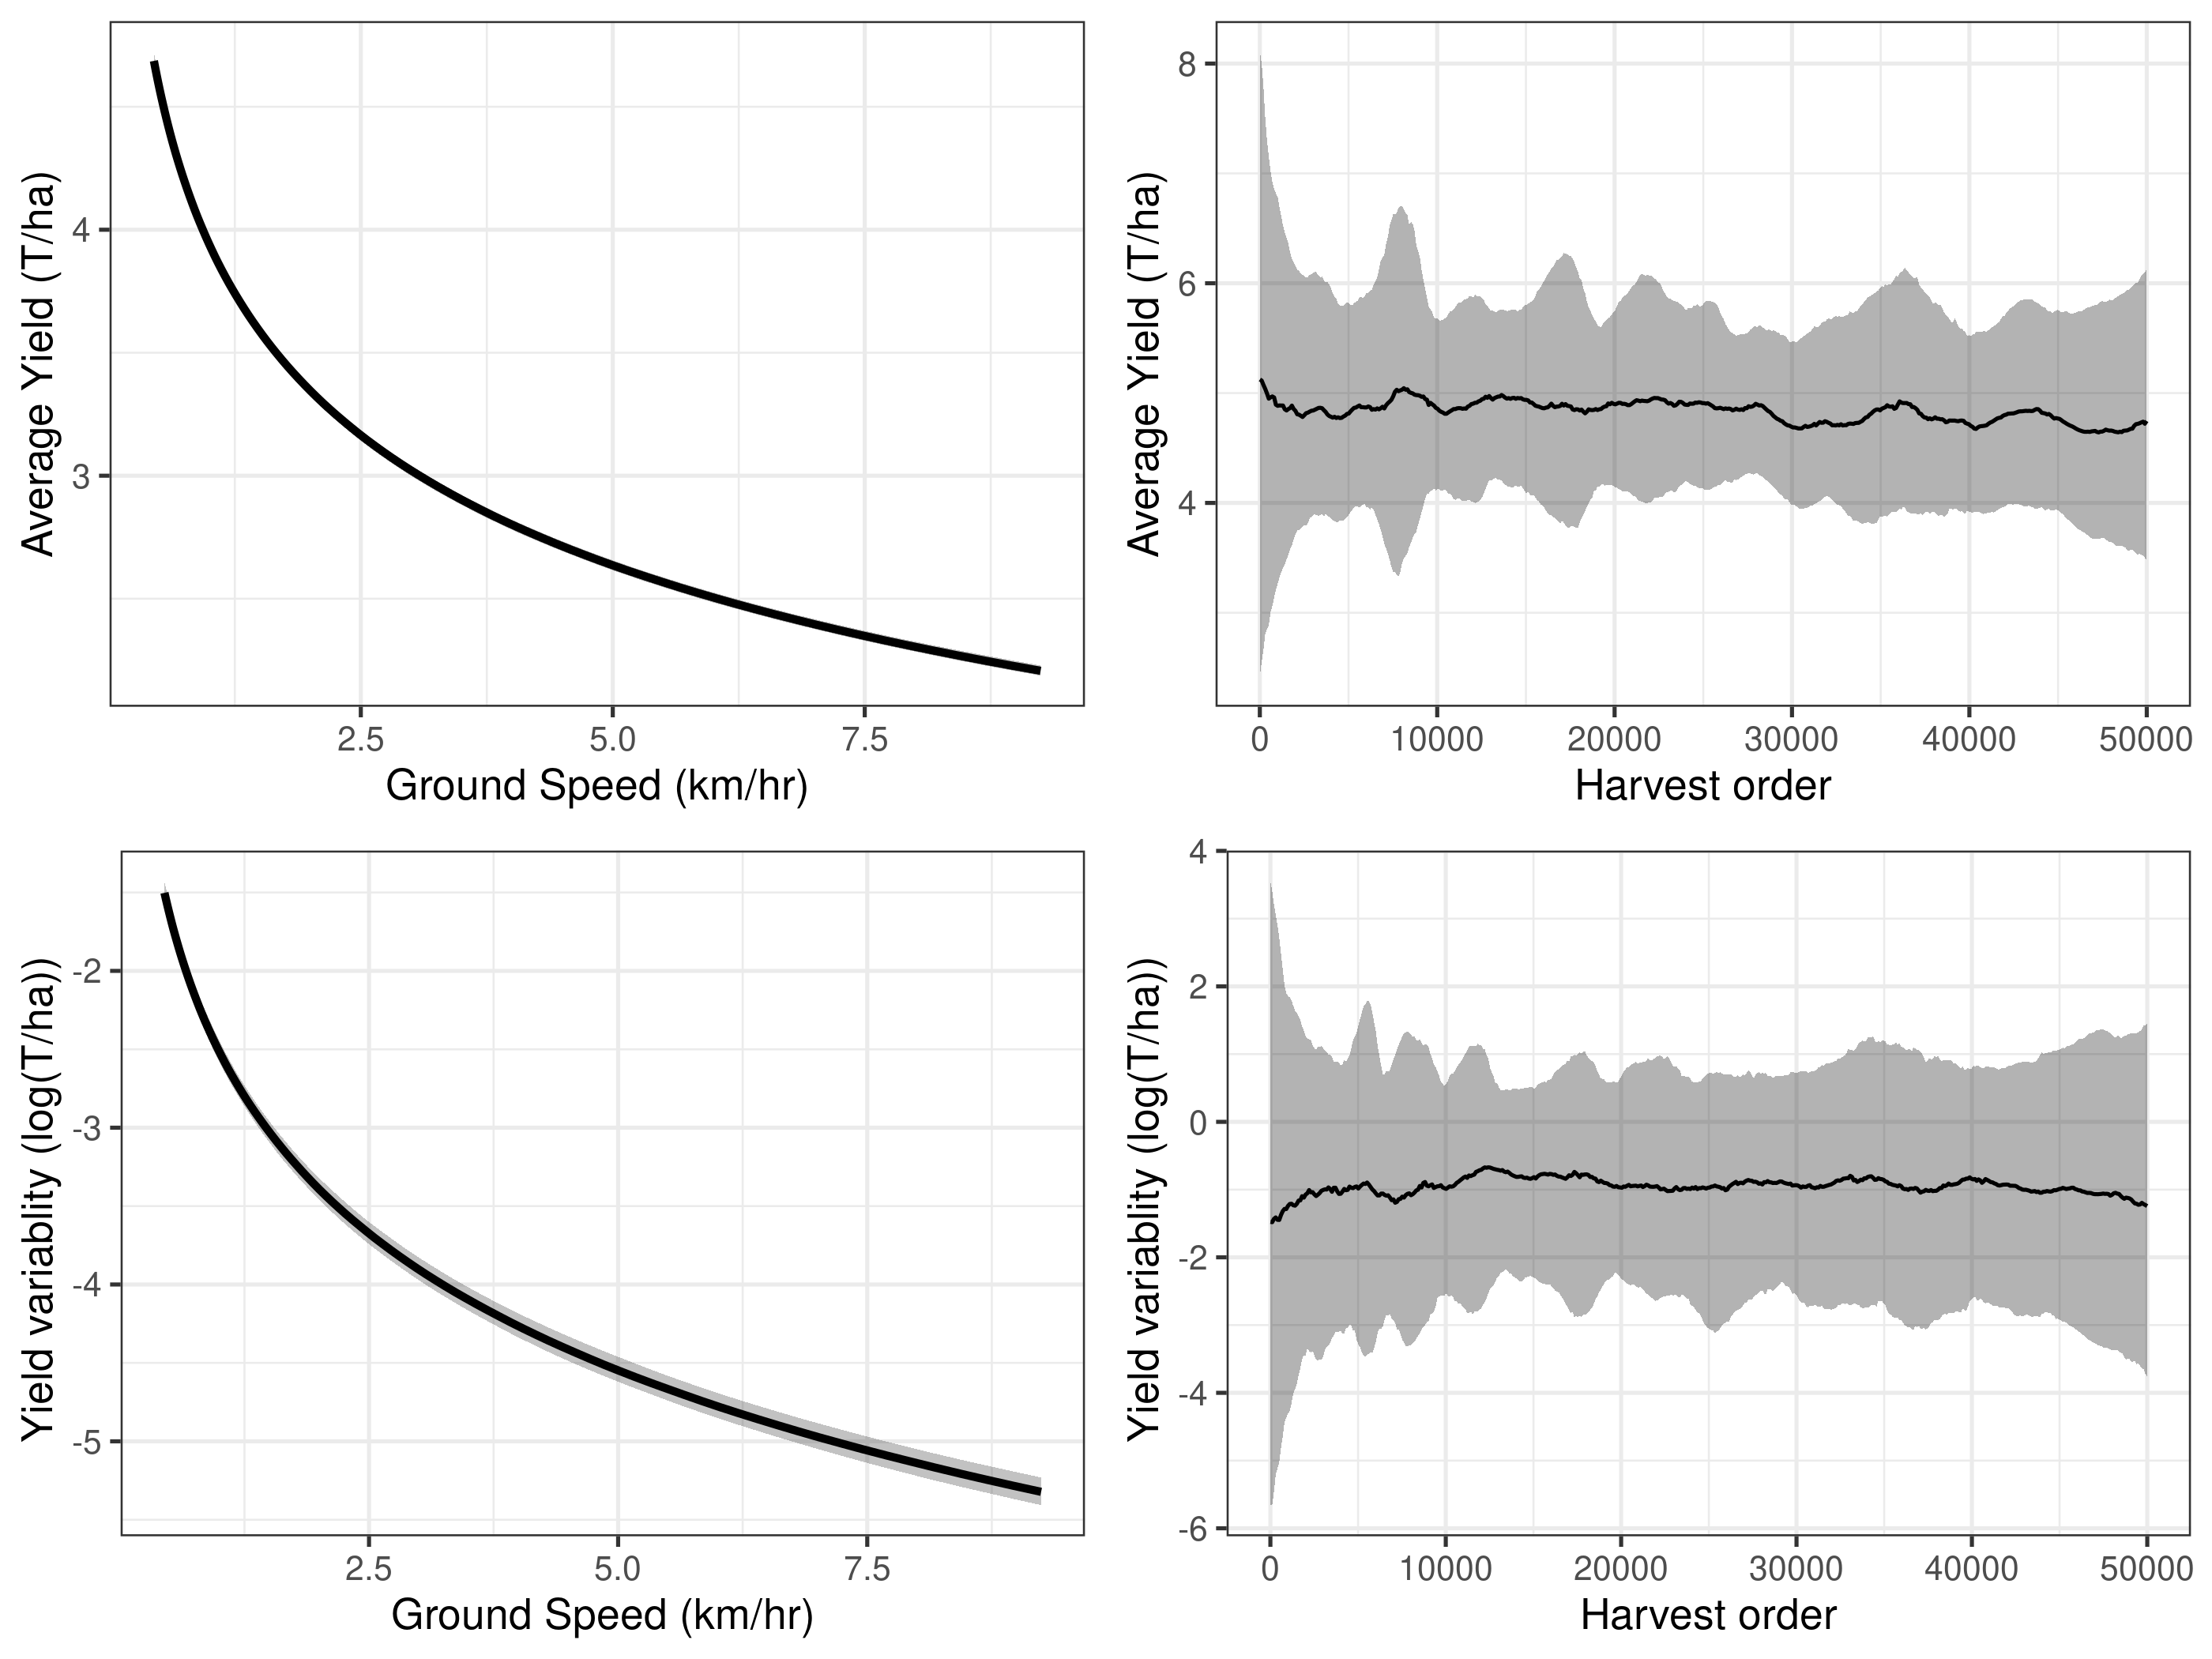
\includegraphics[width=1\linewidth]{../Figures/groundSpeed_canola} \caption{Effect of ground speed and order (sequence of harvest) on canola yield.}\label{fig:canolaPlotSpeed}
\end{figure}

\begin{figure}
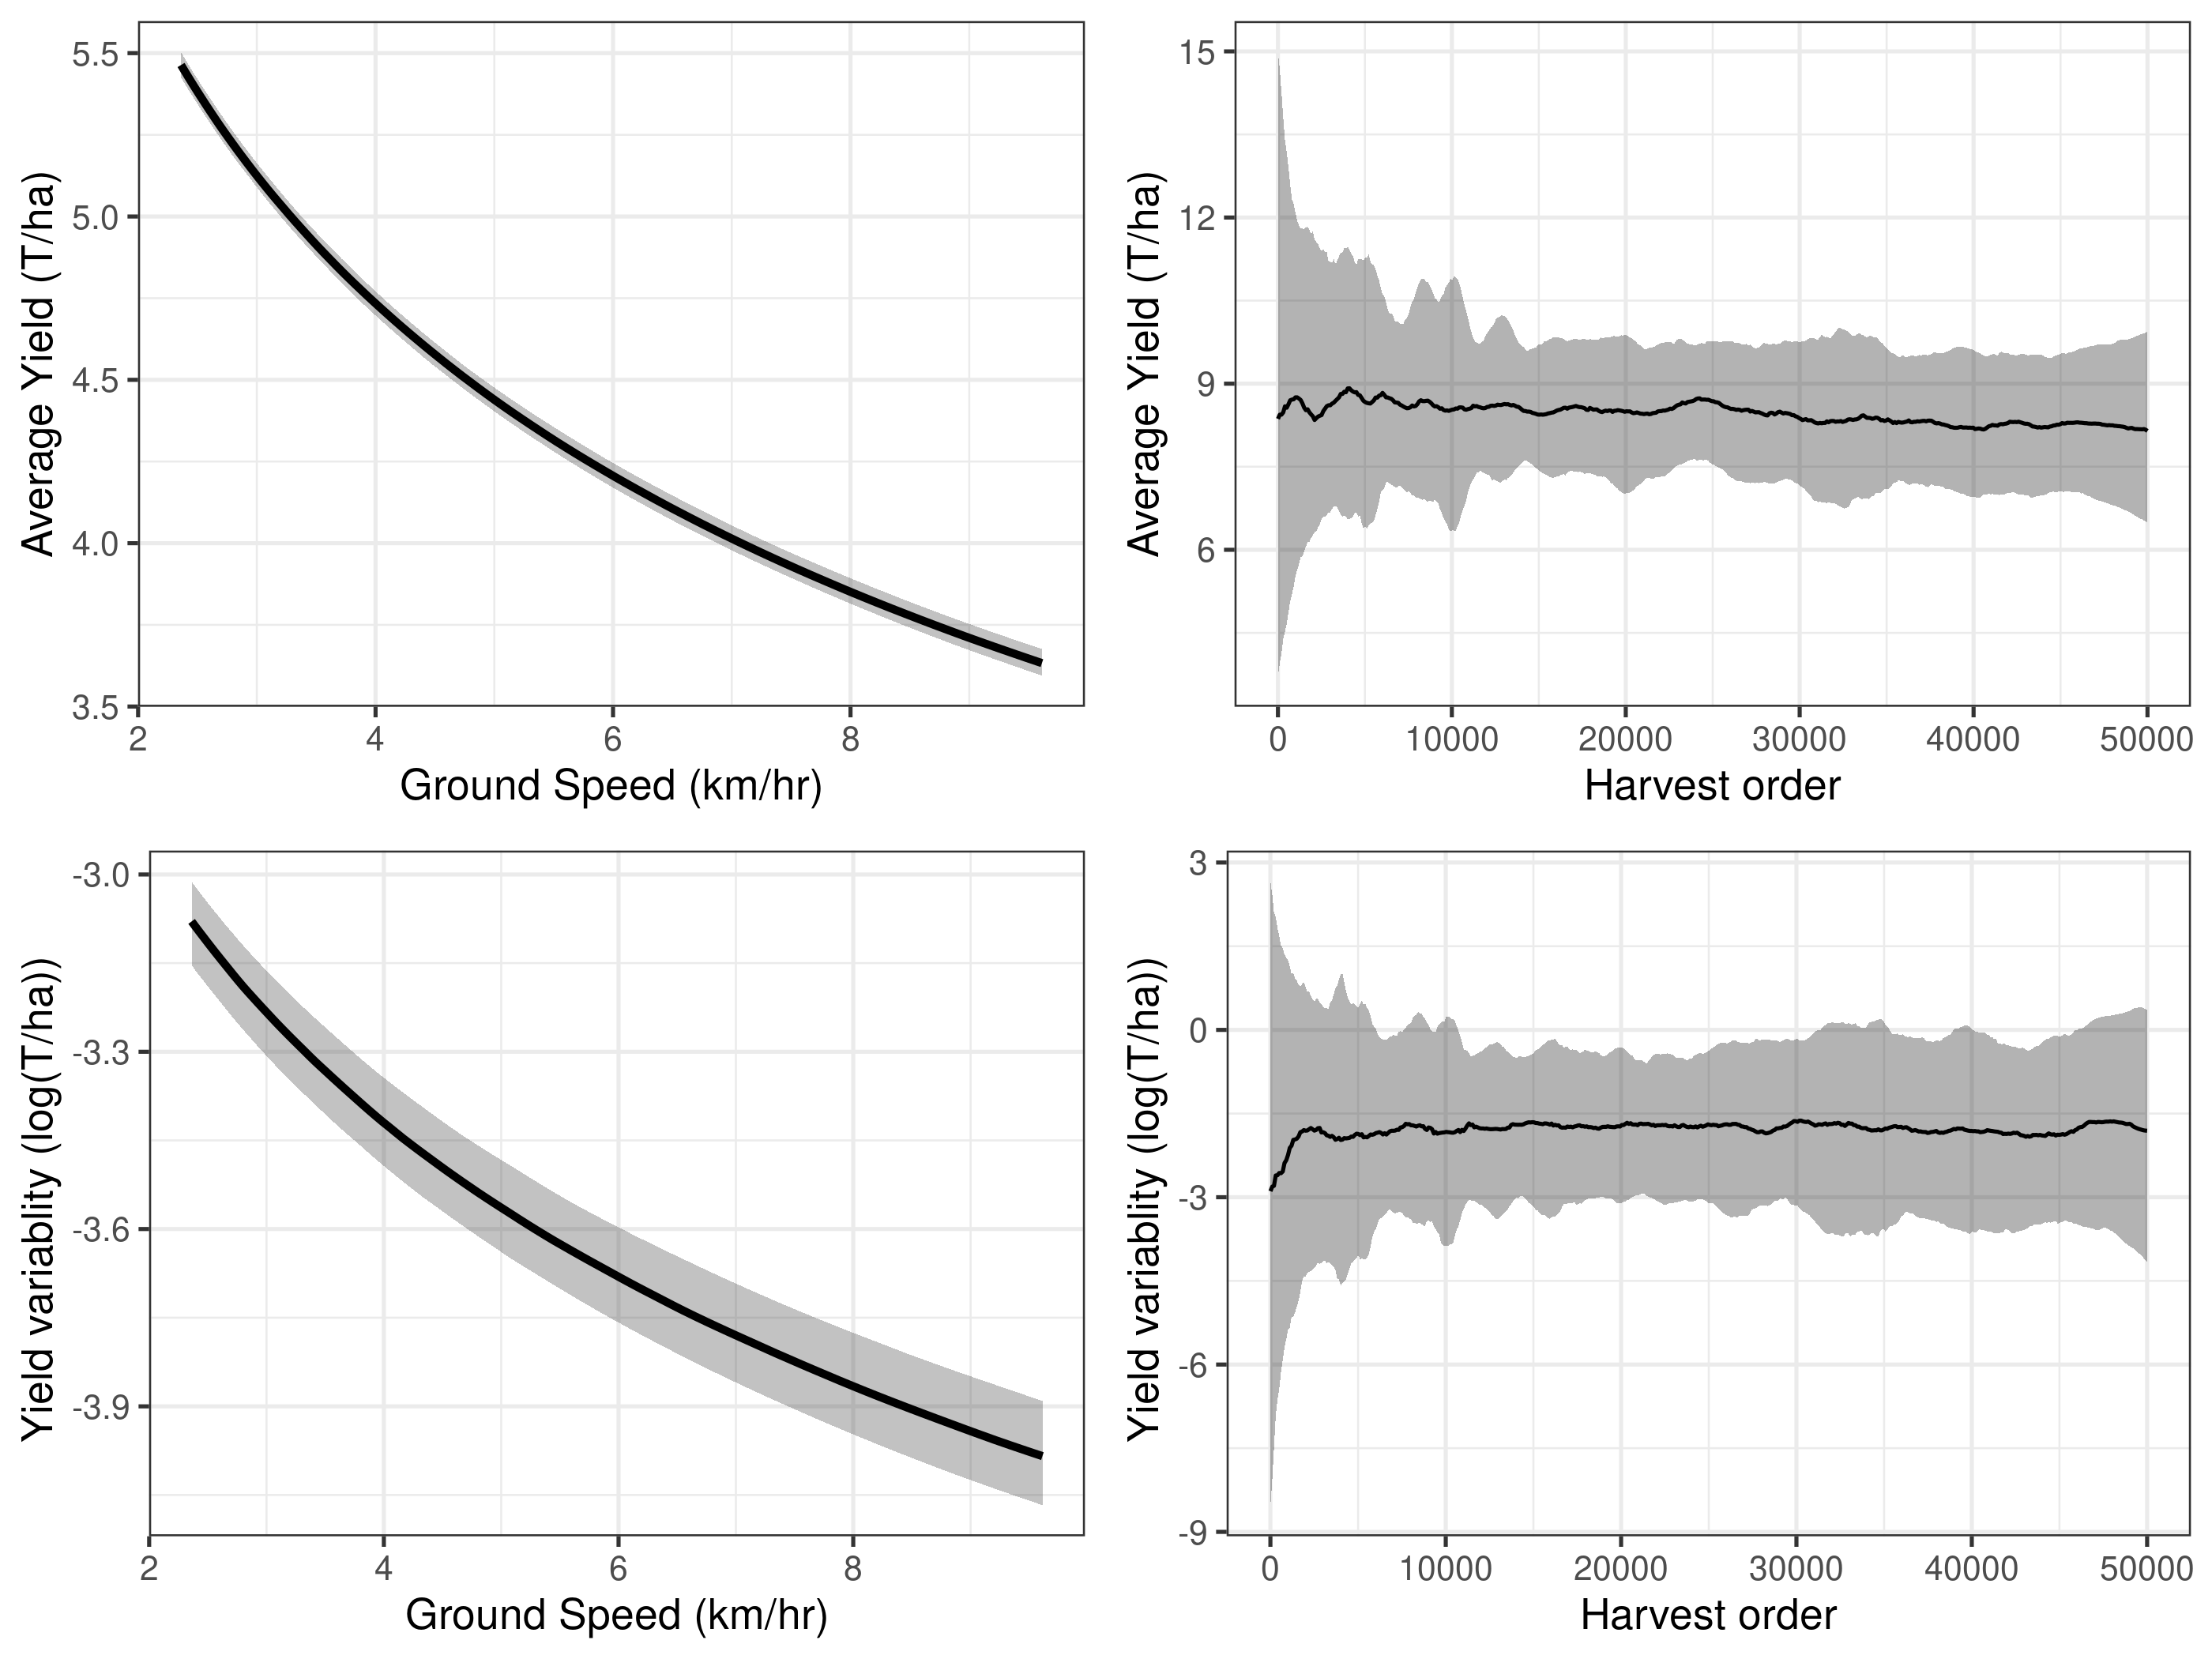
\includegraphics[width=1\linewidth]{../Figures/groundSpeed_wheat} \caption{Effect of ground speed and order (sequence of harvest) on wheat yield.}\label{fig:wheatPlotSpeed}
\end{figure}

\begin{figure}
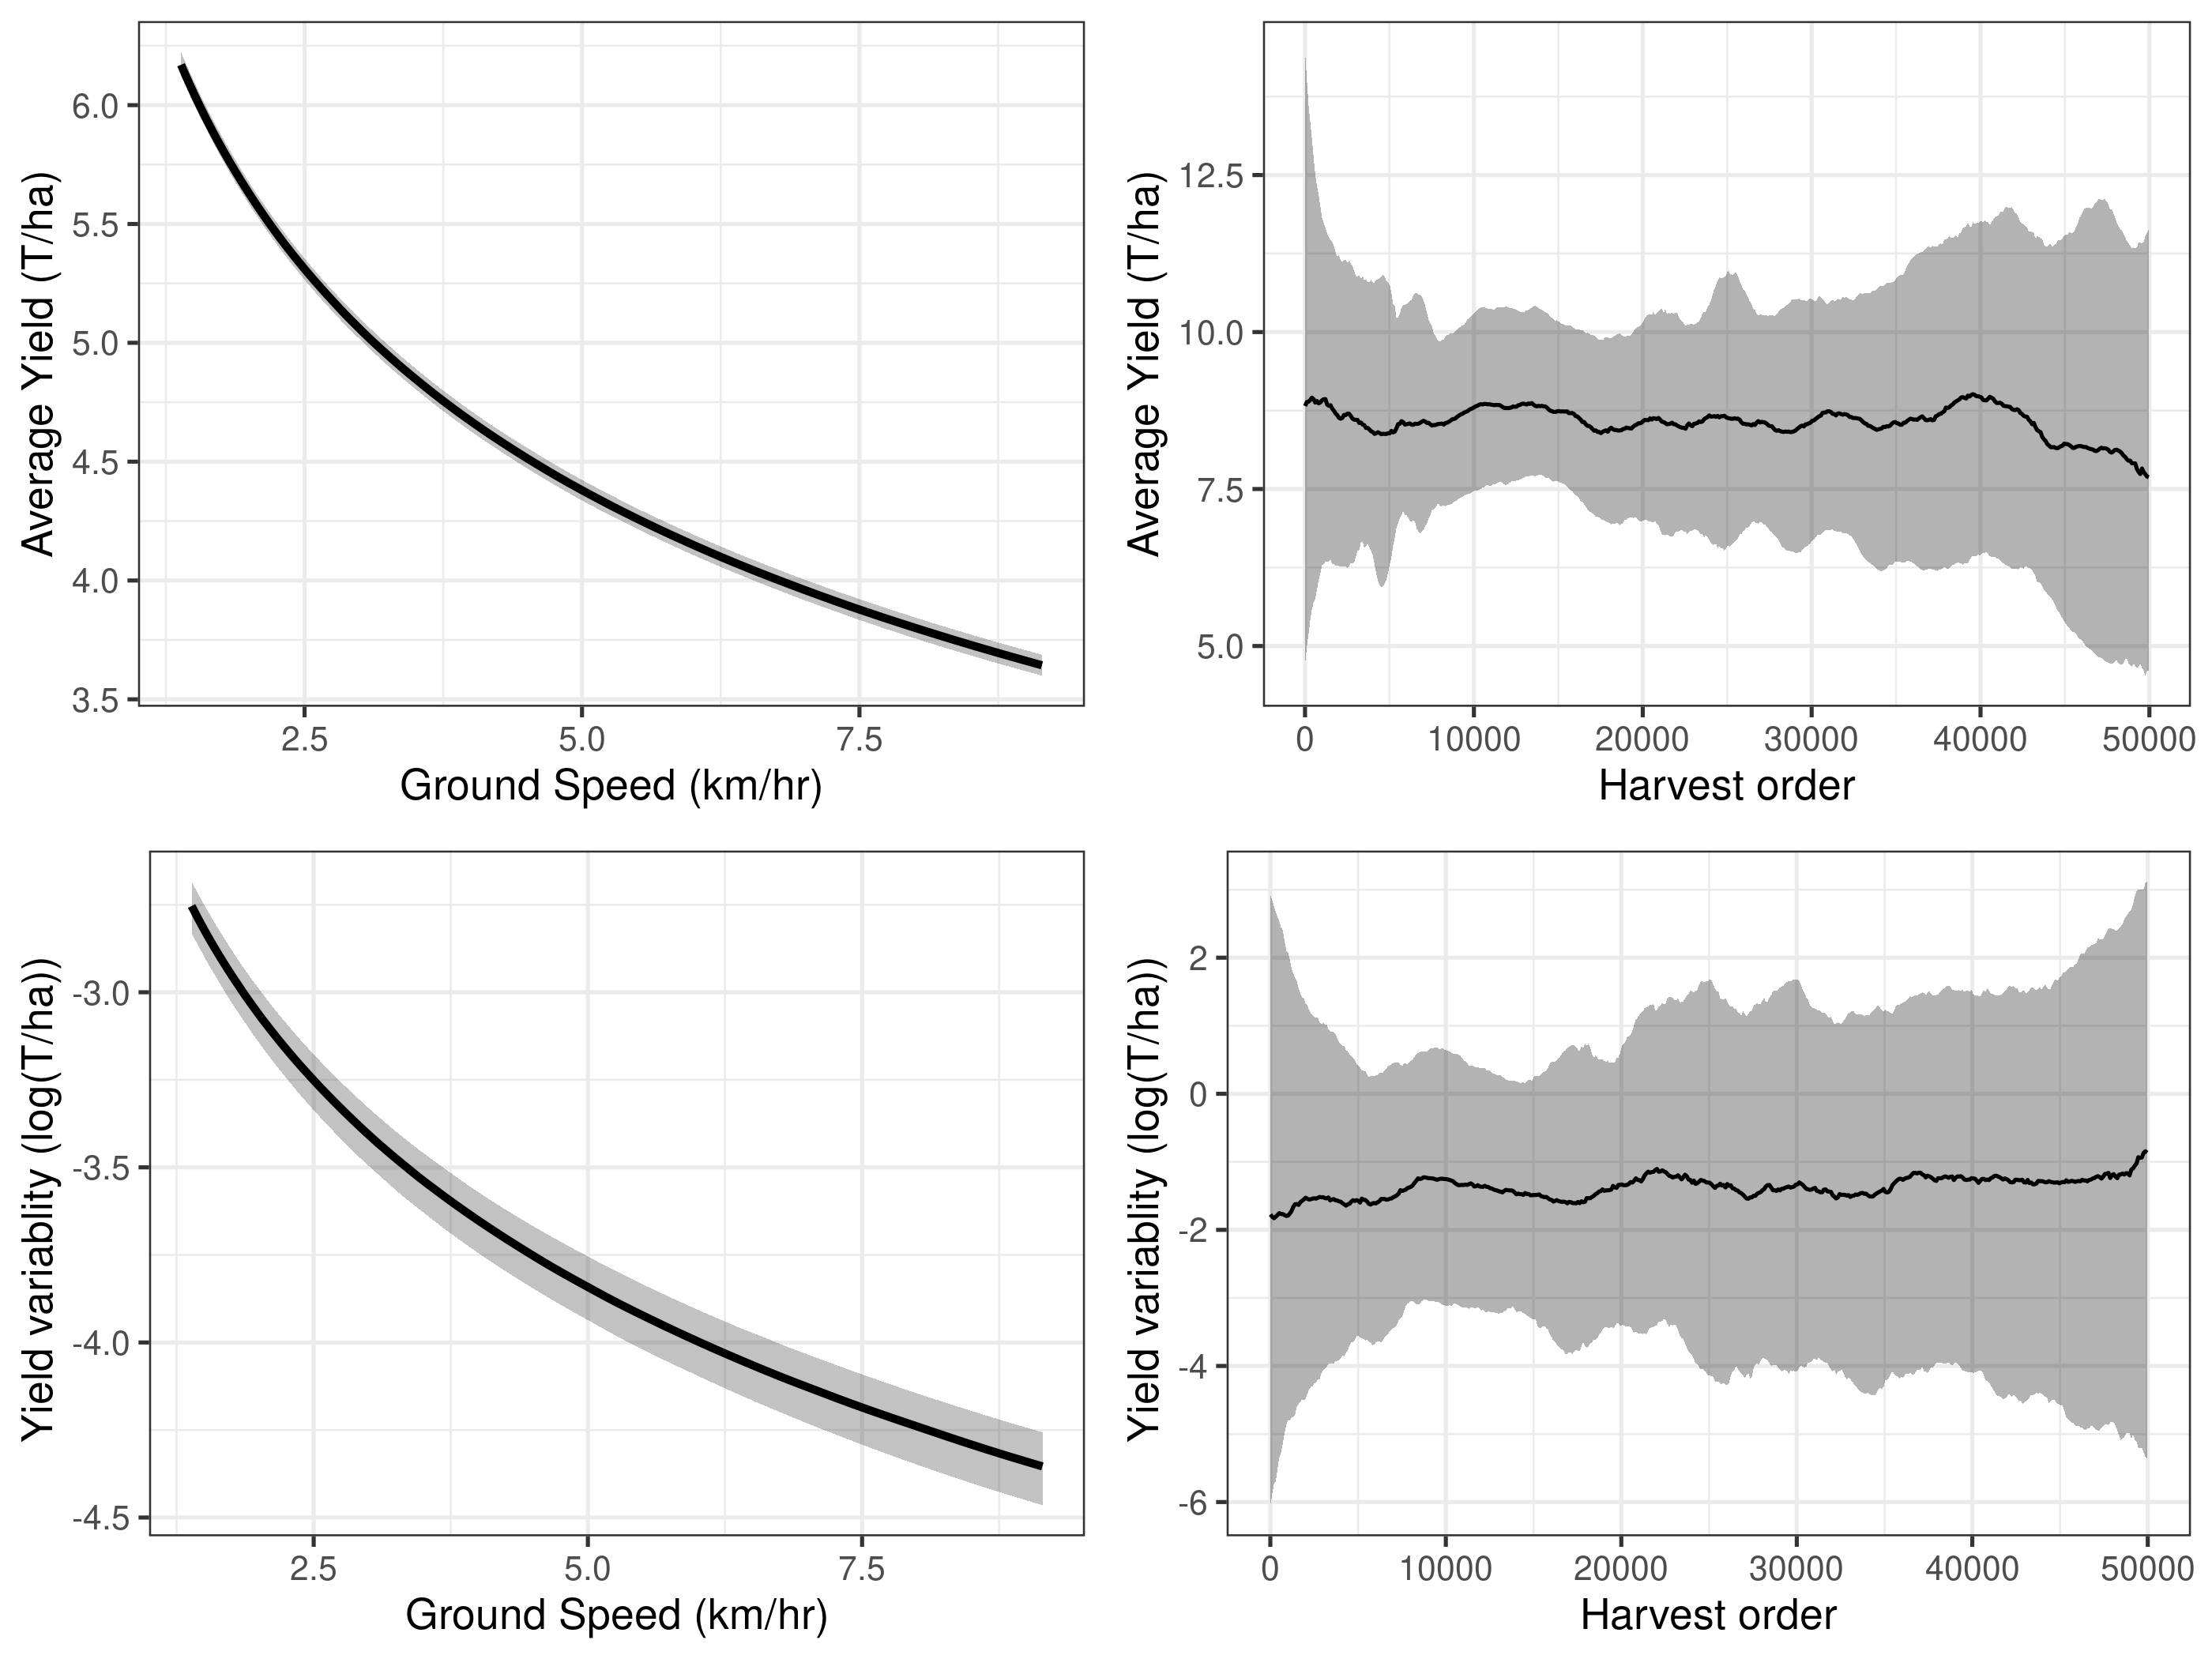
\includegraphics[width=1\linewidth]{../Figures/groundSpeed_peas} \caption{Effect of ground speed and order (sequence of harvest) on pea yield.}\label{fig:peasPlotSpeed}
\end{figure}


\end{document}

